%% Final report: Bipedal Robotic Locomotion with Reinforcement Learning
%% Spring 2026 — Machine Learning course final project
\documentclass[sigconf,nonacm]{acmart}

\usepackage{booktabs}
\usepackage{graphicx}
\graphicspath{{figures/}}

\AtBeginDocument{%
  \providecommand\BibTeX{{%
    \normalfont B\kern-0.5em{\scshape i\kern-0.25em b}\kern-0.8em\TeX}}}

\settopmatter{printacmref=false}
\setcopyright{none}
\renewcommand\footnotetextcopyrightpermission[1]{}
\pagestyle{plain}

\begin{document}

\title{Bipedal Robotic Locomotion with Reinforcement Learning}

\author{Drew Burcher}
\affiliation{%
  \institution{Virginia Tech}
  \city{Blacksburg}
  \state{Virginia}
  \country{USA}}
\email{<TODO: drew@vt.edu>}

\author{Dan Torri}
\affiliation{%
  \institution{Virginia Tech}
  \city{Blacksburg}
  \state{Virginia}
  \country{USA}}
\email{<TODO: dan@vt.edu>}

\author{Nathan Wyatt}
\affiliation{%
  \institution{Virginia Tech}
  \city{Blacksburg}
  \state{Virginia}
  \country{USA}}
\email{<TODO: nathan@vt.edu>}

\renewcommand{\shortauthors}{Burcher, Torri, and Wyatt}

\begin{abstract}
We train a 13-degree-of-freedom bipedal humanoid (Booster Robotics T1) to walk forward in
a PyBullet simulation using two model-free reinforcement learning algorithms:
Soft Actor--Critic (SAC) and Proximal Policy Optimization (PPO). The policy is a
two-layer MLP that maps proprioceptive observations to per-joint position targets,
and a hand-shaped reward combines forward velocity, an alive bonus, an energy cost,
and several stability penalties. After roughly 2.8\,M environment steps the SAC
policy reaches a mean evaluation return of about 7{,}100 and a forward speed of
$\sim$1.6\,m/s, while PPO under several reward variants plateaus near a return of
3{,}000 and never produces a sustained gait. We discuss the reward-shaping decisions
that drove these results, the catastrophic-forgetting failures we saw with SAC late
in training, and the practical trade-offs between on- and off-policy methods on a
dense-reward locomotion task.
\end{abstract}

\keywords{reinforcement learning, bipedal locomotion, humanoid robot, SAC, PPO, PyBullet}

\maketitle

% ====================================================================
\section{Introduction}
% ====================================================================
Getting a bipedal robot to walk is a classic test bed for control because the
system is high-dimensional, underactuated, and unstable in its natural rest
state---small mistakes early in a step quickly cascade into a fall. Classical
controllers exist for this problem (zero-moment-point trackers, model-predictive
control, quadratic-programming whole-body controllers), but they all require
fairly accurate dynamics models and careful tuning, and the resulting gaits tend
to be brittle outside their design point.

Reinforcement learning offers an attractive alternative: instead of writing down
a controller, we specify what we want (move forward, stay upright, save energy)
and let an optimizer search policy space for behaviors that maximize that
reward. Modern actor--critic methods such as SAC~\cite{haarnoja2018sac} and
PPO~\cite{schulman2017ppo} have made this practical, and a number of recent
papers~\cite{rudin2022learn,siekmann2021sim2real} have shown that policies
trained entirely in simulation can transfer to physical hardware.

In this project we work in simulation only, on the Booster Robotics T1 humanoid,
and use the project as a hands-on comparison of two of the most widely used
deep-RL algorithms. Concretely we ask:

\begin{enumerate}
\item Can either SAC or PPO learn a stable forward gait on the T1 from scratch
  using a simple proprioceptive state and a dense, hand-shaped reward?
\item How does the off-policy method (SAC) compare to the on-policy method
  (PPO) in terms of sample efficiency, wall-clock training time, final
  performance, and stability of the learned policy?
\item Which reward terms actually shape the gait, and which are easy for the
  policy to ``hack'' into degenerate behaviors?
\end{enumerate}

The remainder of the paper is organized as follows. Section~\ref{sec:related}
surveys related work on learned locomotion. Section~\ref{sec:method} describes
the simulator, the observation/action spaces, the reward, and our SAC and PPO
configurations. Section~\ref{sec:results} reports the training curves, an
ablation of reward components, and qualitative observations of the learned
gait. Section~\ref{sec:conclusion} concludes and lists what we would do
differently with more time. The contribution statement is in
Section~\ref{sec:contributions}.

% ====================================================================
\section{Related Work}\label{sec:related}
% ====================================================================
\textbf{Classical bipedal control.} Most ``walking robot'' demos before the
deep-learning era use either trajectory-tracking controllers built around
zero-moment-point analysis~\cite{kajita2003zmp} or model-predictive whole-body
controllers~\cite{koenemann2015whole}. These work well when the robot model is
accurate, but require non-trivial engineering to keep the robot stable on
uneven ground or under disturbances.

\textbf{Deep RL for locomotion.} Schulman et al.\ introduced
PPO~\cite{schulman2017ppo} as a stable, easy-to-tune on-policy method, and it
quickly became the default for continuous-control benchmarks such as MuJoCo's
\textit{Humanoid}, \textit{Walker2d} and \textit{HalfCheetah}. Haarnoja et
al.~\cite{haarnoja2018sac} proposed SAC, which adds an entropy term to the
objective and uses an off-policy replay buffer; on dense-reward continuous
tasks it is typically more sample efficient than PPO at the cost of more
complex implementation and more sensitive temperature tuning.

\textbf{Sim-to-real bipeds.} Siekmann et al.~\cite{siekmann2021sim2real} train
PPO policies in MuJoCo and deploy them on the Cassie biped, using domain
randomization and a periodic reward to encourage stepping. Rudin et
al.~\cite{rudin2022learn} train massively parallel PPO policies for the ANYmal
quadruped in NVIDIA Isaac Gym, demonstrating that scaling up rollouts can
matter more than algorithm choice. Peng et al.~\cite{peng2018deepmimic} showed
that imitation rewards from motion-capture data dramatically reduce the search
problem for humanoid characters; we deliberately do not use motion data here so
we can study what the algorithms find on their own.

\textbf{Simulators and tooling.} Our environment is built on
PyBullet~\cite{coumans2016pybullet} and wrapped in a Gymnasium~\cite{gymnasium}
interface, and we use the Stable-Baselines3~\cite{raffin2021sb3}
implementations of SAC and PPO so the comparison reflects standard
implementations rather than algorithmic differences hidden in our own code.

% ====================================================================
\section{Method}\label{sec:method}
% ====================================================================

\subsection{Robot and simulator}
The Booster Robotics T1 is a $\sim$1.2\,m humanoid with 23 revolute joints. We
load its URDF in PyBullet and run physics at 240\,Hz. The two head joints are
locked, and the eight arm joints are held at zero by a stiff position
controller, so the policy controls the remaining 13 joints (waist plus six per
leg: hip pitch/roll/yaw, knee pitch, and ankle pitch/roll). Locking the arms
keeps the action space small and removes a common reward-hacking strategy
(spinning the arms for ``forward velocity'' from the torso).

The policy runs at 60\,Hz, so each policy step advances four 240\,Hz physics
sub-steps. Episodes last up to 1{,}000 policy steps ($\sim$16.7\,s). An
episode terminates early if the torso drops below 0.35\,m, rises above 2\,m
(launched), or tilts past $\sim$70\textdegree~in roll or pitch.

\subsection{Observation and action spaces}
The observation is a 36-dim float vector concatenating: torso height (1),
torso orientation as Euler angles (3), torso linear and angular velocity (3+3),
and the 13 actuated joint positions and velocities (13+13). We deliberately
exclude global $x,y$ position so the policy is translation-invariant.

The action $a\in[-1,1]^{13}$ is a normalized joint-angle target. We map it to
each joint's URDF limits and apply position control through PyBullet's
\texttt{POSITION\_CONTROL} mode with PD gains $K_p{=}0.2,\,K_d{=}0.5$. The
ankles use softer/more damped gains ($K_p{=}0.1,\,K_d{=}1.0$) because we found
high-stiffness ankles cause the foot to chatter against the ground and
introduce a large energy penalty for no behavioral benefit.

\subsection{Reward function}
We use a dense, hand-tuned reward applied at every policy step. With
$\dot{x}$ the torso forward velocity, $\tau$ the joint torques, $\dot{q}$ the
joint velocities, $\phi,\theta$ the torso roll and pitch, $q_i$ the joint
angles relative to their normalized [-1,1] range, and $\dot{z}$ the torso
vertical velocity:
\begin{align}
r_t \;=\; & 3.0\,\dot{x} && \text{forward velocity} \nonumber \\
        + & 2.0 && \text{alive bonus} \nonumber \\
        - & 0.00495\,\overline{|\tau\cdot\dot{q}|} && \text{energy} \nonumber \\
        - & 0.5\,(\phi^2+\theta^2) && \text{torso upright} \nonumber \\
        - & 0.2\sum_i \max(|q_i|-0.5,\,0)^2 && \text{joint limits} \nonumber \\
        - & 0.5\,\max(-\dot{z},0) && \text{anti-drop} \nonumber
\end{align}
A one-time penalty of $-100$ is added on episode termination by falling. The
forward-velocity reward is intentionally linear and unbounded so the policy is
always rewarded for moving faster, and the energy term is small enough that it
becomes important only after the policy has learned to walk (Fig.\
\ref{fig:reward-mag}). The joint-limit term is a quadratic ramp that only kicks
in past 50\% of the joint range so it does not interfere with normal motion.

\subsection{RL algorithms}
We use the Stable-Baselines3~\cite{raffin2021sb3} implementations of SAC and
PPO with a shared $[256,256]$ MLP for actor and critic, $\gamma{=}0.99$, and
Adam at $3\!\times\!10^{-4}$. SAC uses a 1\,M-transition replay buffer, batch
size 256, soft target updates with $\tau{=}0.005$, and auto-tuned entropy with
target entropy $-5$. PPO uses 2{,}048 rollout steps, 10 SGD epochs, batch size
64, GAE $\lambda{=}0.95$, clip range 0.2, value coefficient 0.5, and entropy
bonus 0.01. Both algorithms run on CPU; for our network sizes and batch sizes
this was about 2$\times$ faster than CUDA in our setup, mostly because the
PyBullet step is the bottleneck rather than the gradient update.

\subsection{Training infrastructure}
We wrote a thin training harness around Stable-Baselines3 that (i) auto-commits
the source tree to git before each run so any policy can be re-derived,
(ii) writes a JSON metadata file with the full hyperparameter set and reward
weights, (iii) runs a deterministic 5-episode evaluation every 5{,}000 steps and
records a GIF of the last evaluation, and (iv) renders a live matplotlib
dashboard alongside the PyBullet GUI so we could watch the robot and the
training curves at the same time. Total training time for the SAC run reported
here was approximately 12 hours of wall clock across multiple sessions on a
single laptop.

% ====================================================================
\section{Results and Evaluation}\label{sec:results}
% ====================================================================
We focus on a single long SAC run (\texttt{sac\_legs\_only\_v5}, 2.8\,M
environment steps after warm-up, accumulating across resumed sessions for a
total of $\sim$5.5\,M trained transitions) and several shorter PPO runs spanning
the same wall-clock budget. Every plot in this section is produced from the
JSON metrics dumped by our training harness.

\subsection{SAC: learning curves}
Figure~\ref{fig:learning-curve} shows the per-episode return for SAC. The
policy spends roughly 300\,k steps just learning to stand, then transitions
into a clear walking phase between 1.0\,M and 2.0\,M steps, and finally
plateaus around an episode return of 6{,}000 with occasional collapses. The
deterministic evaluation curve (Fig.\ \ref{fig:eval-curve}, mean over 5
evaluation episodes with action noise disabled) is smoother and reaches
$\sim$7{,}100, indicating that most of the variance in the training curve
comes from the stochastic policy's exploration, not from the underlying
behavior.

\begin{figure}[t]
  \centering
  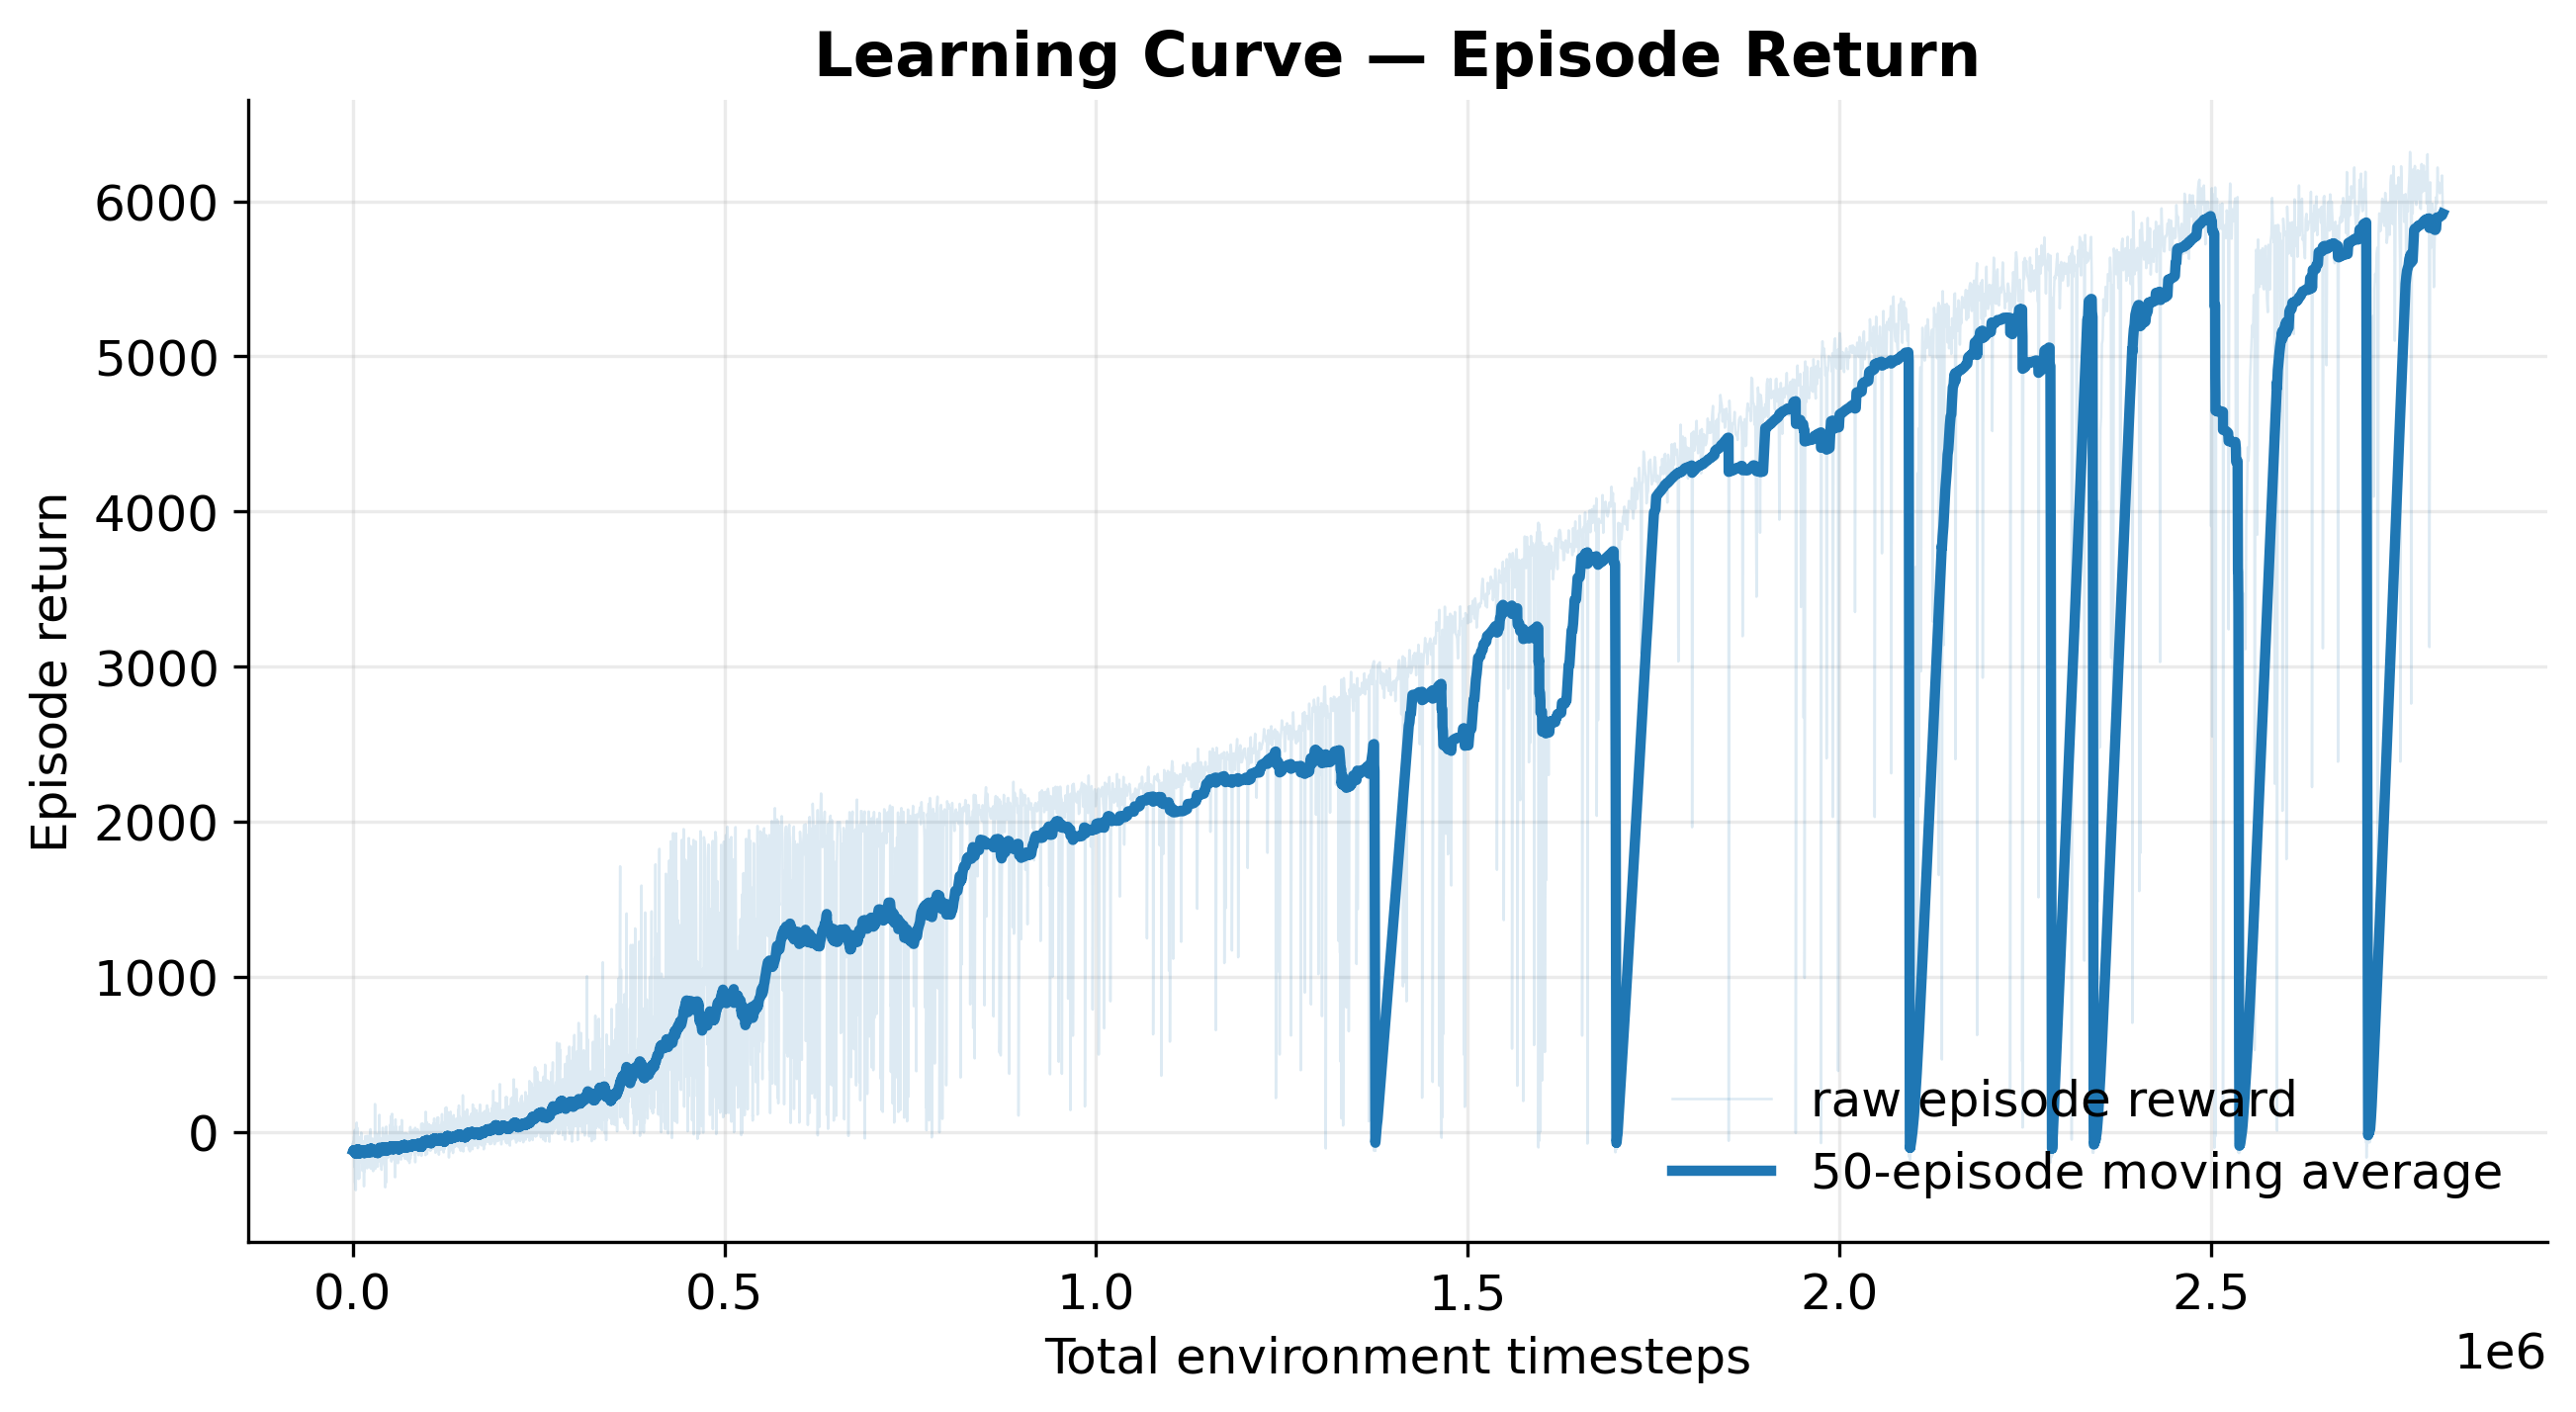
\includegraphics[width=\linewidth]{01_learning_curve.png}
  \caption{SAC training return per episode (light) with 50-episode moving
  average (dark). Sharp dips after 1.4\,M steps correspond to brief catastrophic
  forgetting events.}
  \label{fig:learning-curve}
\end{figure}

\begin{figure}[t]
  \centering
  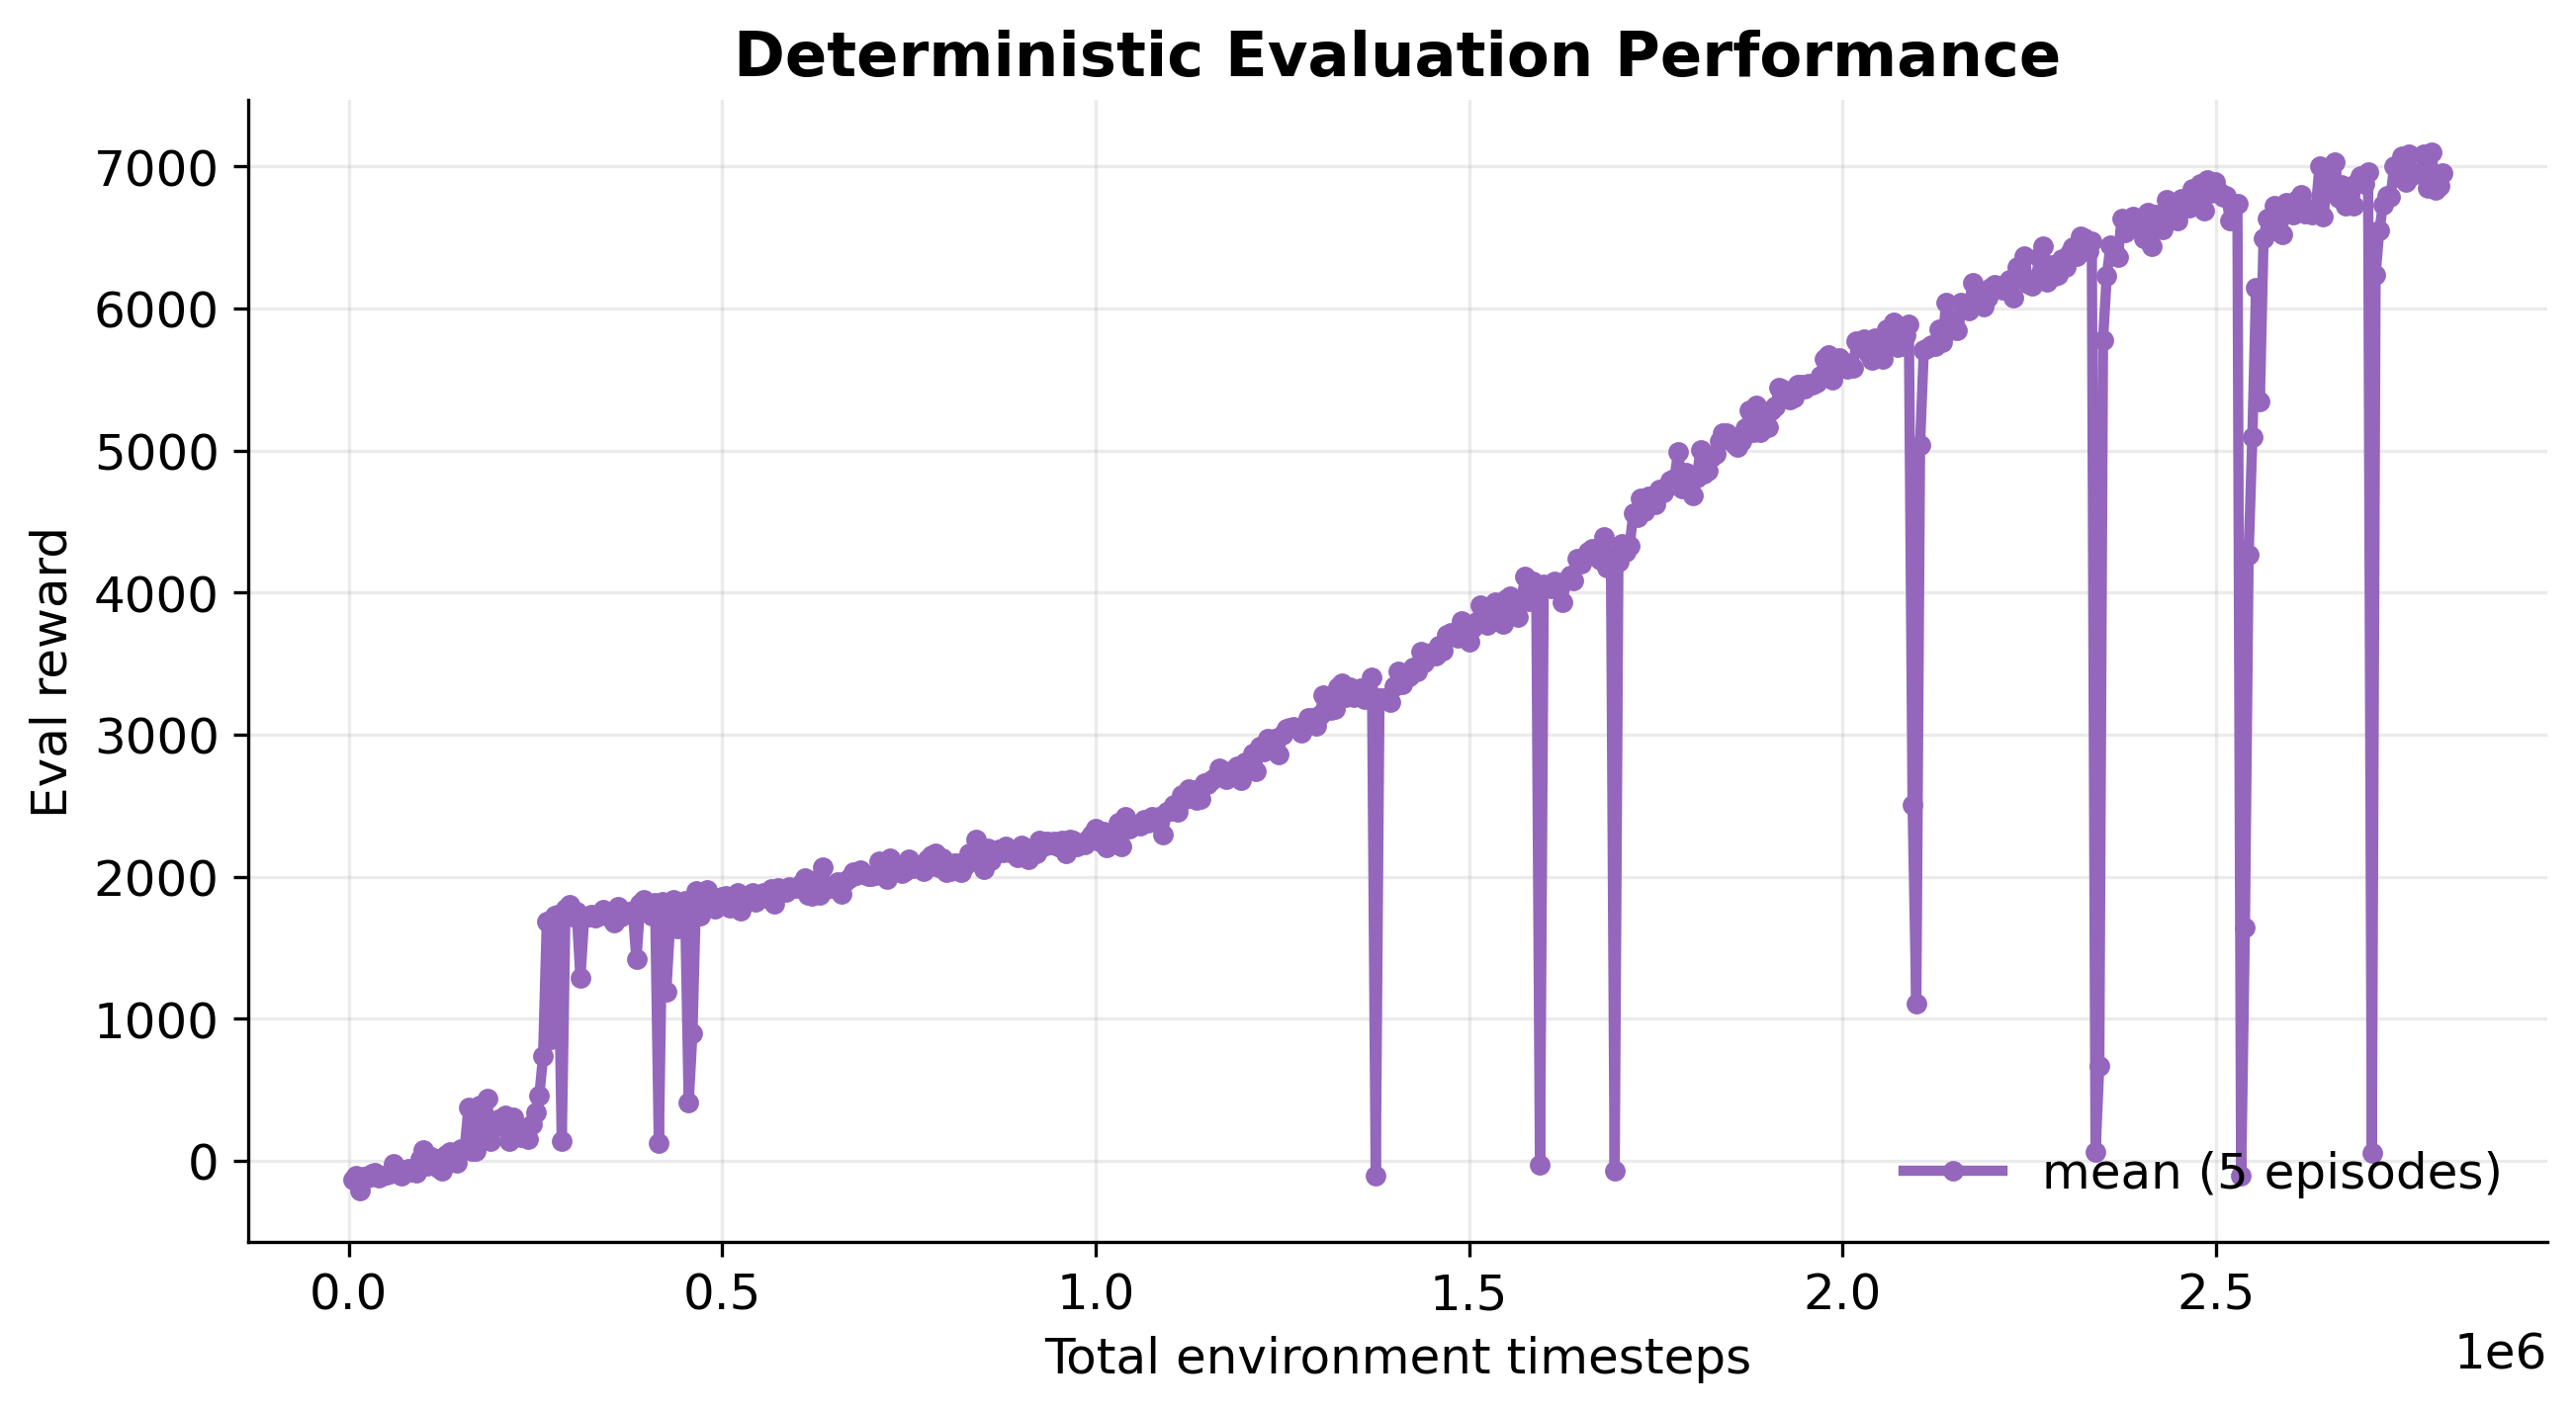
\includegraphics[width=\linewidth]{03_eval_performance.png}
  \caption{Deterministic evaluation return (mean over 5 episodes, action noise
  disabled). The curve is smoother than the training return because exploration
  noise is removed, and it crosses 7{,}000 by 2.6\,M steps.}
  \label{fig:eval-curve}
\end{figure}

\subsection{From standing to walking}
Figure~\ref{fig:survival} shows episode length (capped at 1{,}000) and
Figure~\ref{fig:speed} shows mean forward velocity. Together they illustrate
the two phases of learning: (1) keep the robot from falling for the entire
episode, which the policy nails by about 1\,M steps, and (2) actually move
forward, which only ramps up after standing is solved. By 2.8\,M steps the
policy walks at $\sim$1.6\,m/s and travels $\sim$26\,m per 16.7\,s episode
(Fig.\ \ref{fig:distance}), a brisk walking pace for a robot of this scale.

\begin{figure}[t]
  \centering
  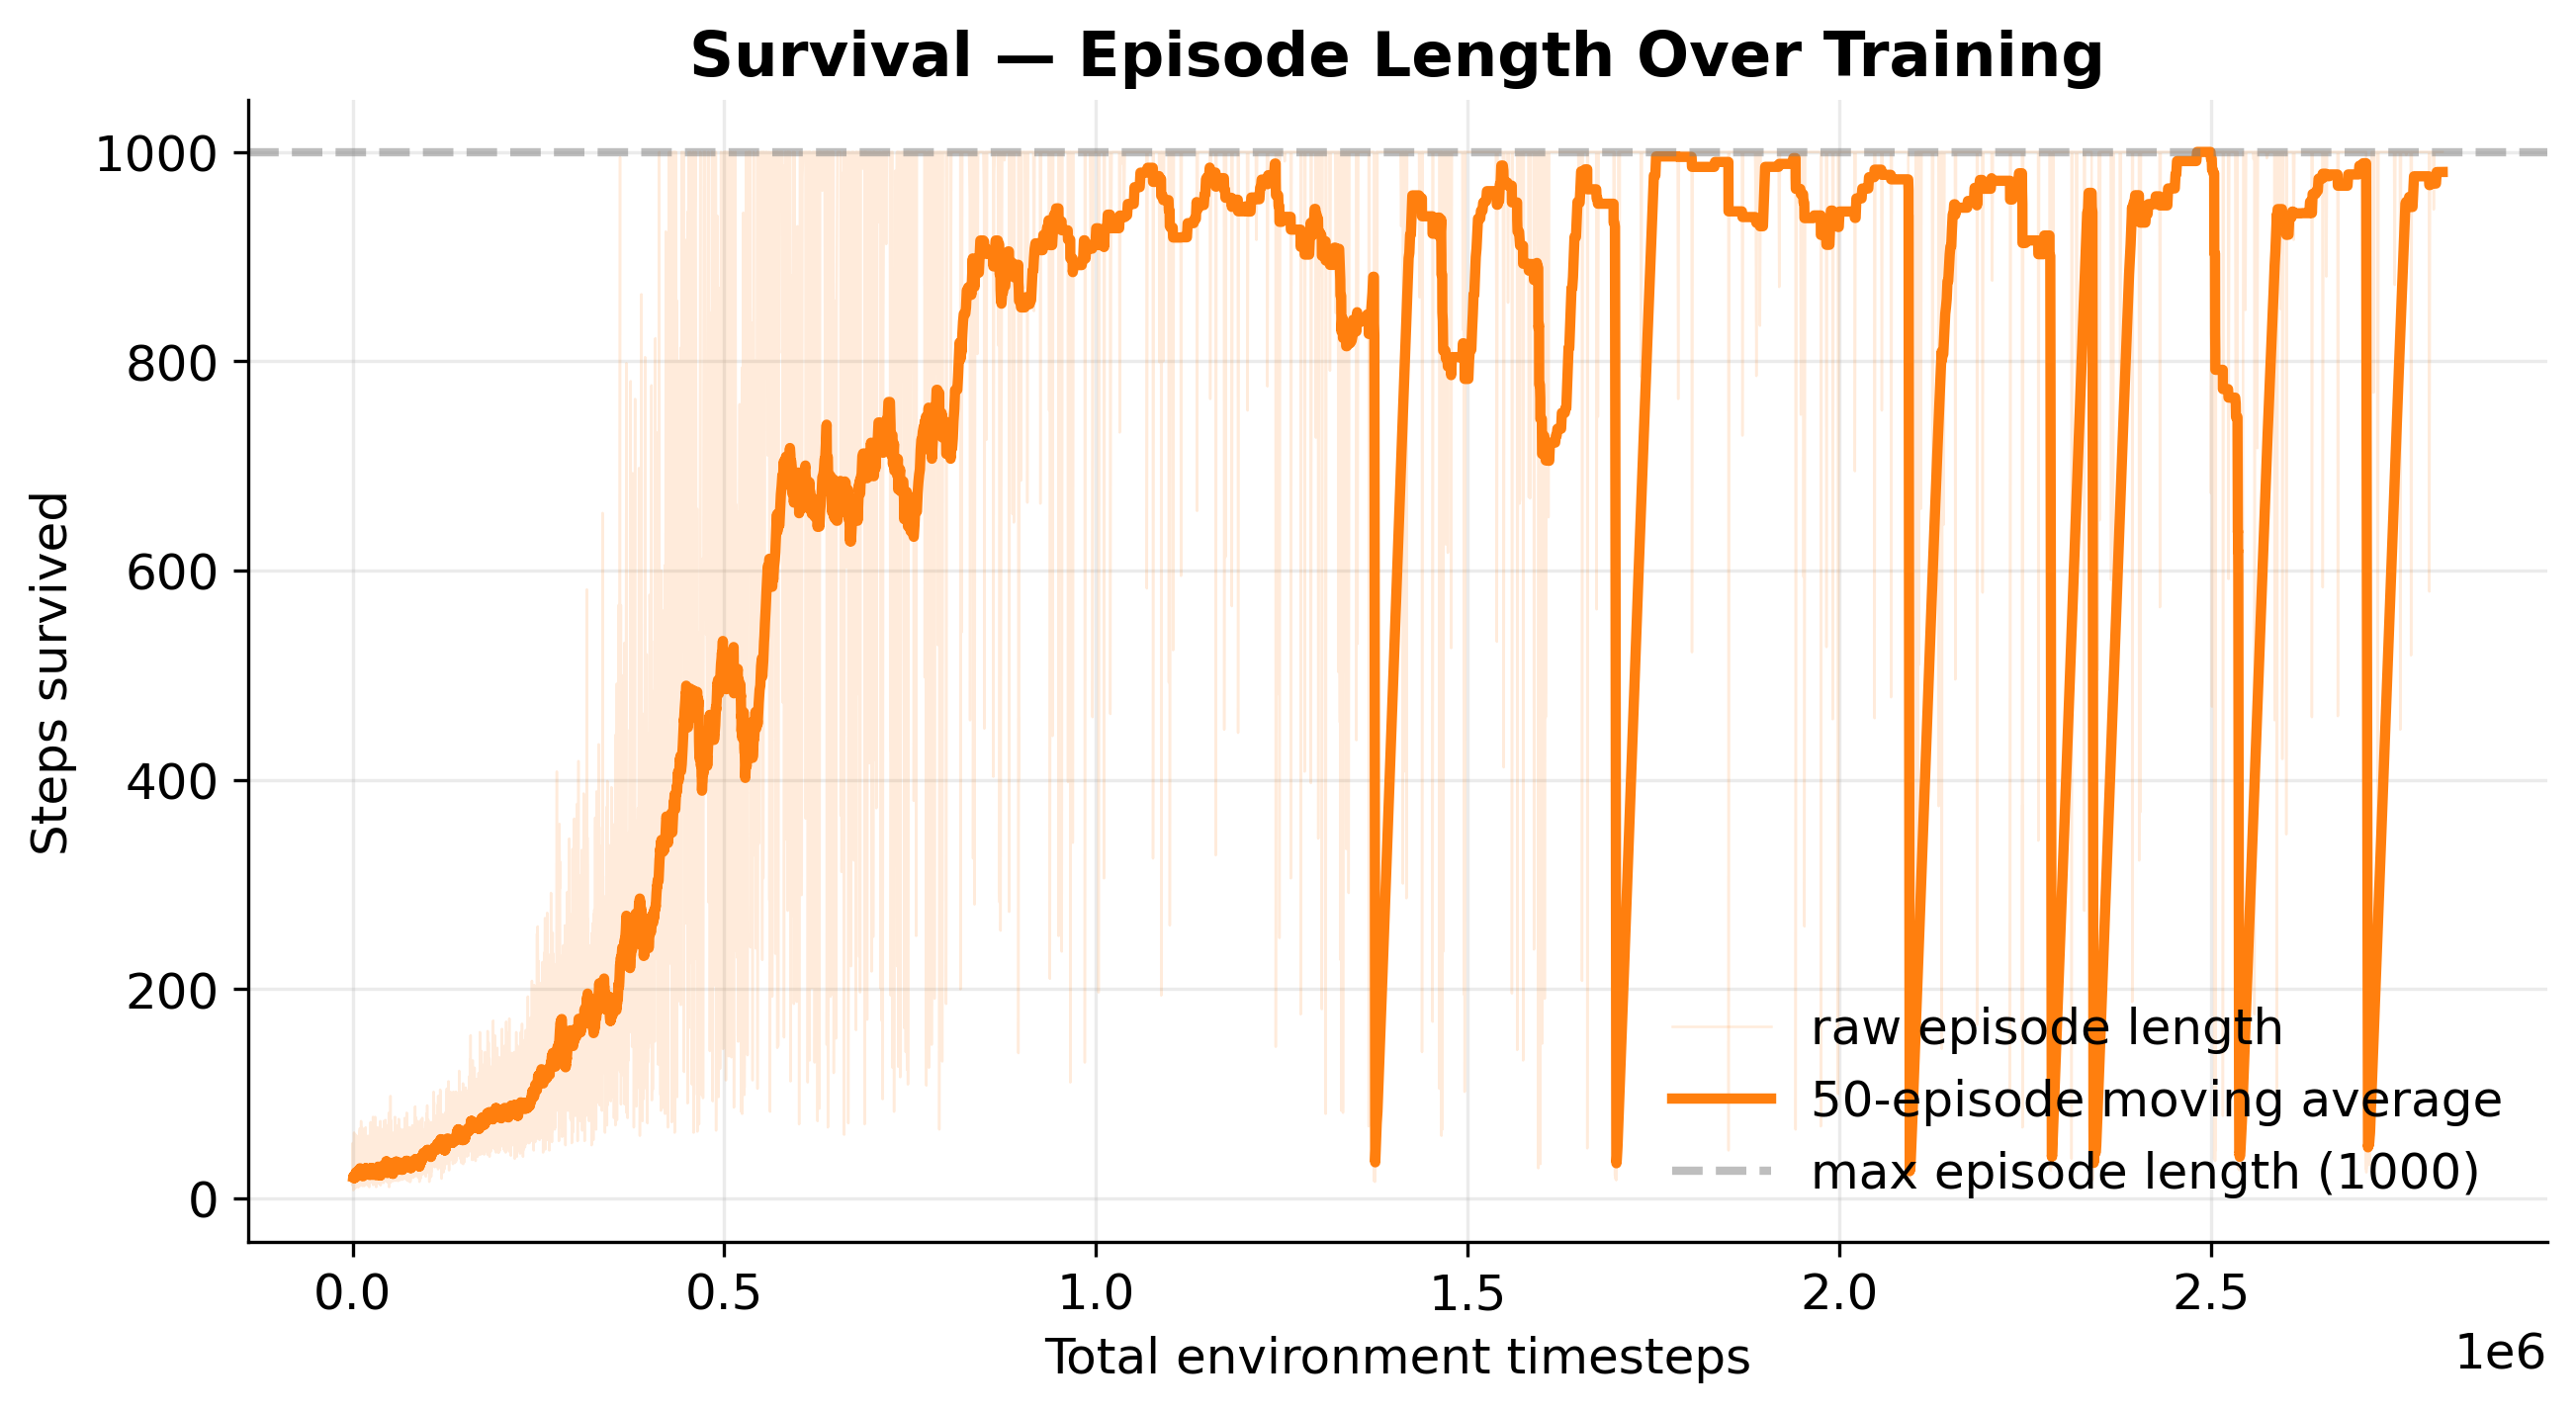
\includegraphics[width=\linewidth]{02_episode_length.png}
  \caption{Episode length (steps survived). The 1{,}000 ceiling is reached
  reliably after $\sim$1.0\,M steps; the dips later in training match the
  catastrophic-forgetting events visible in Fig.~\ref{fig:learning-curve}.}
  \label{fig:survival}
\end{figure}

\begin{figure}[t]
  \centering
  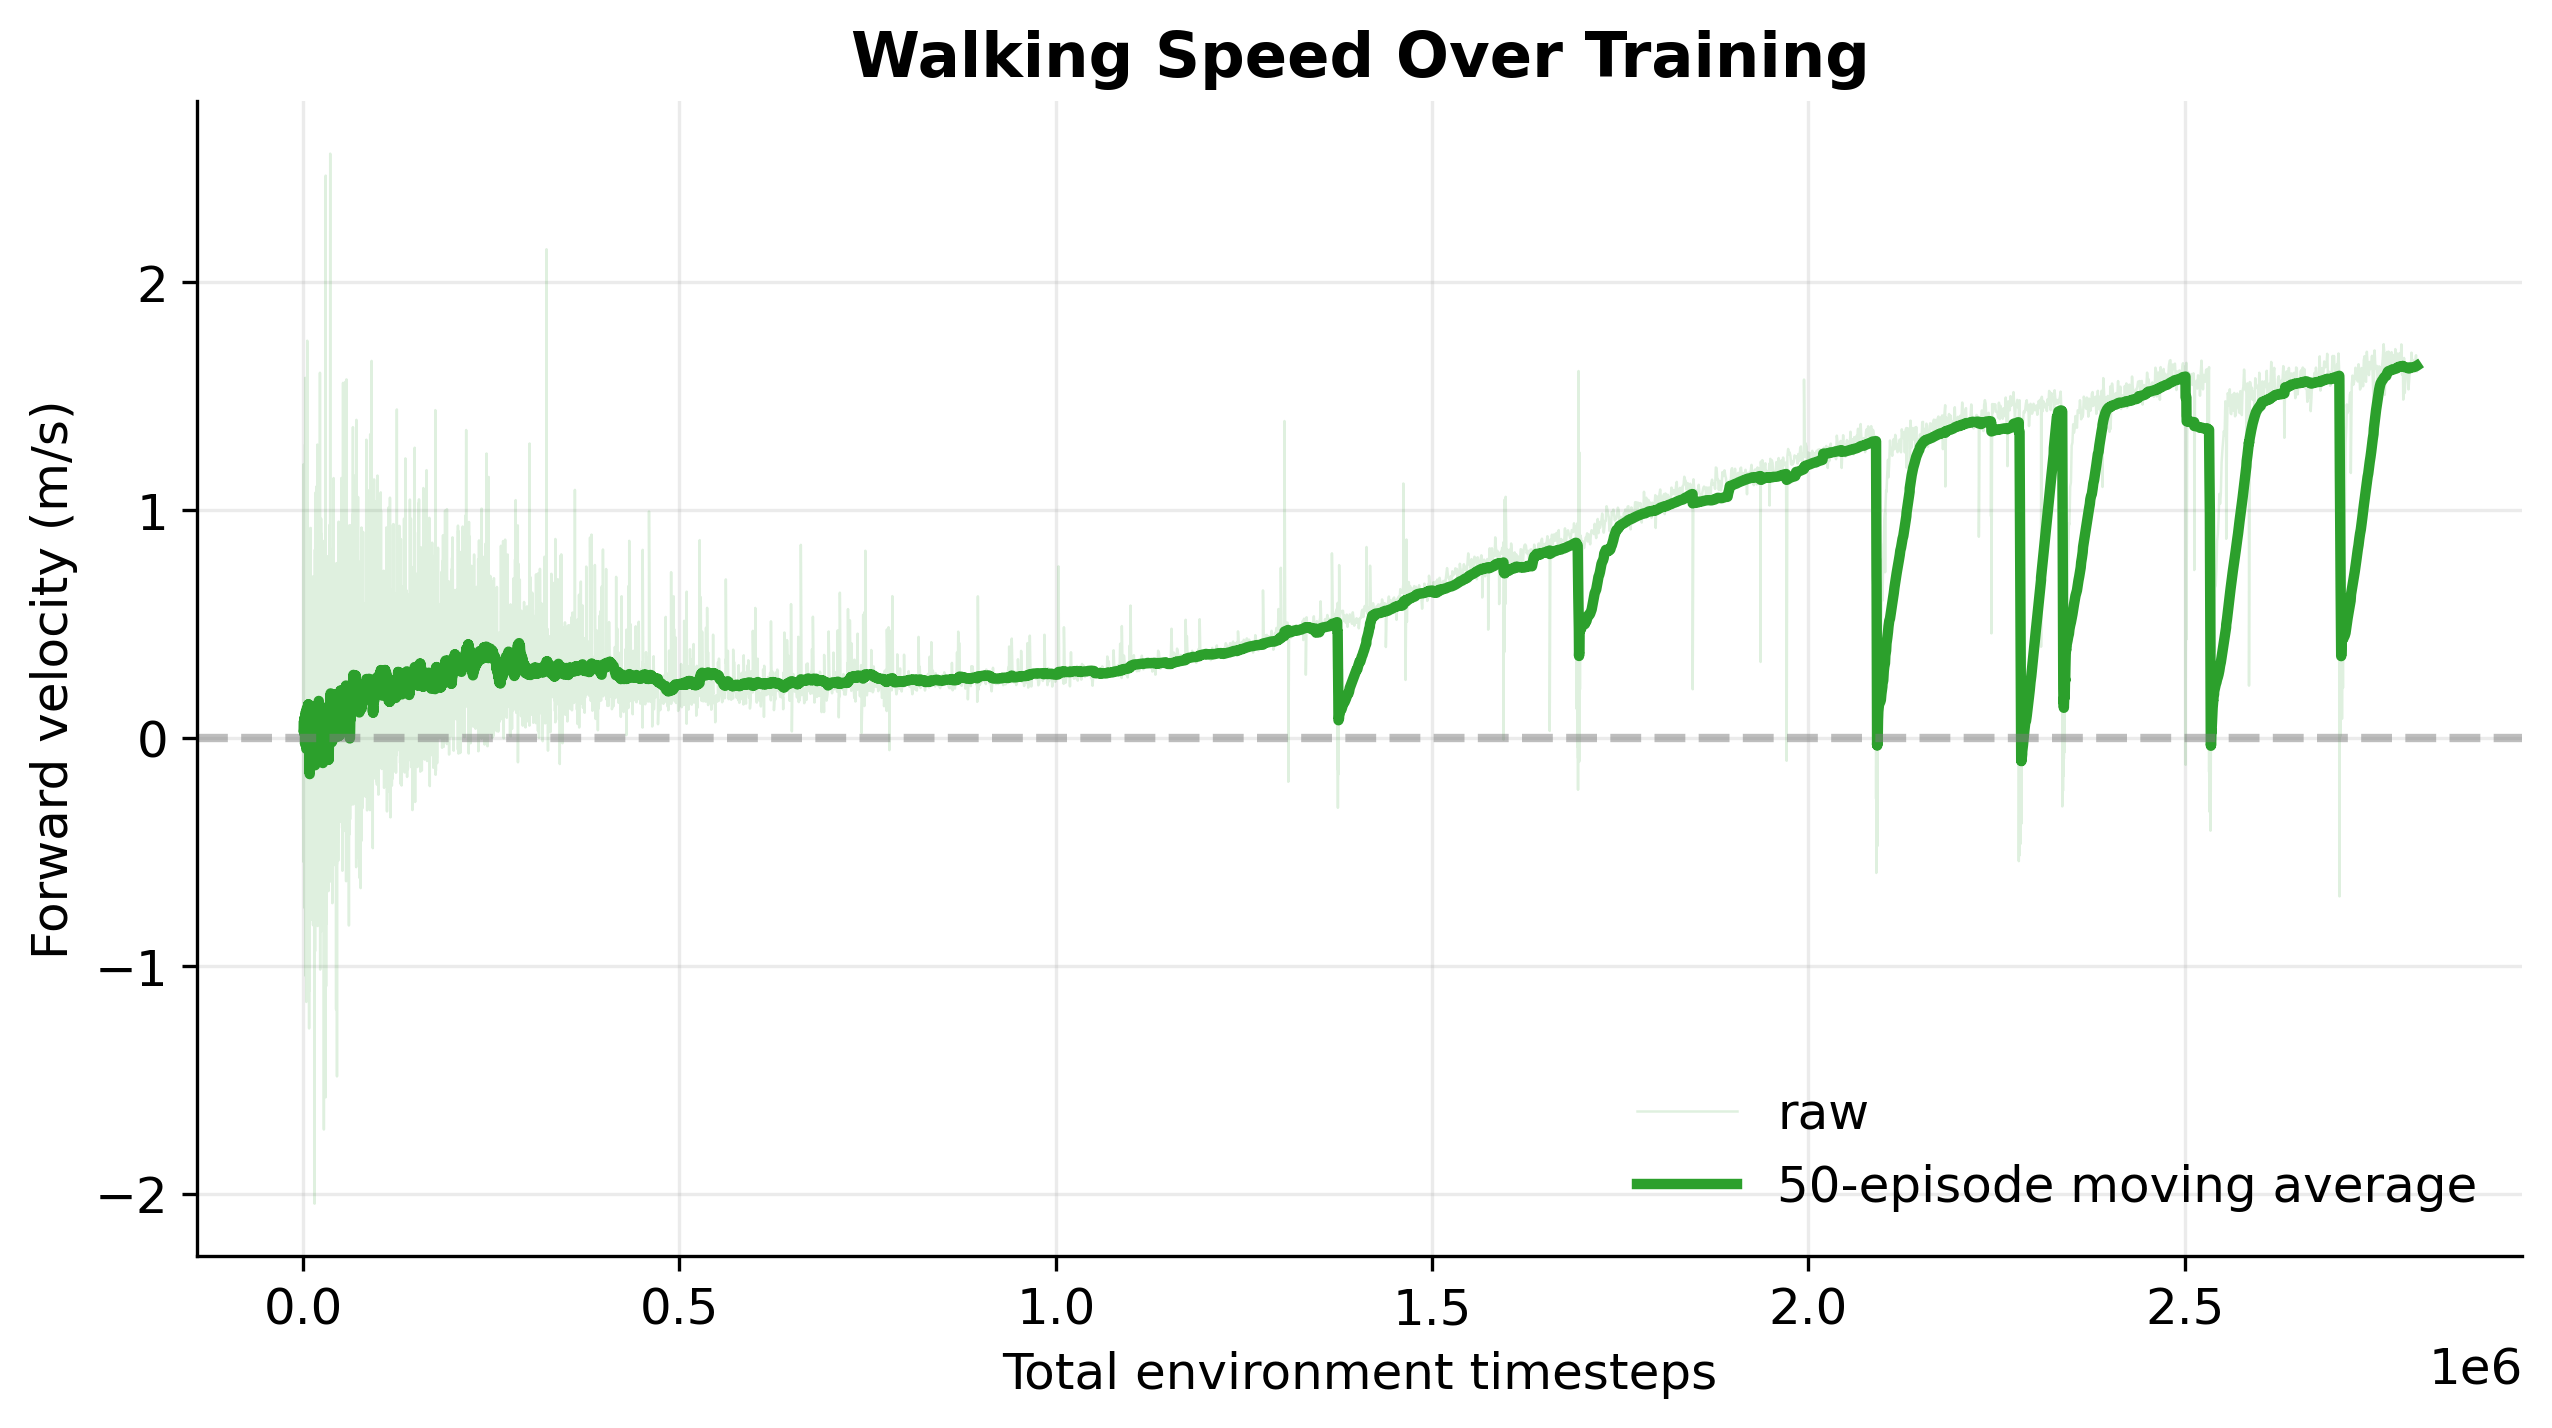
\includegraphics[width=\linewidth]{04_forward_velocity.png}
  \caption{Mean forward torso velocity per episode. The policy is essentially
  stationary until 1.0\,M steps and then accelerates roughly linearly with
  training to $\sim$1.6\,m/s.}
  \label{fig:speed}
\end{figure}

\begin{figure}[t]
  \centering
  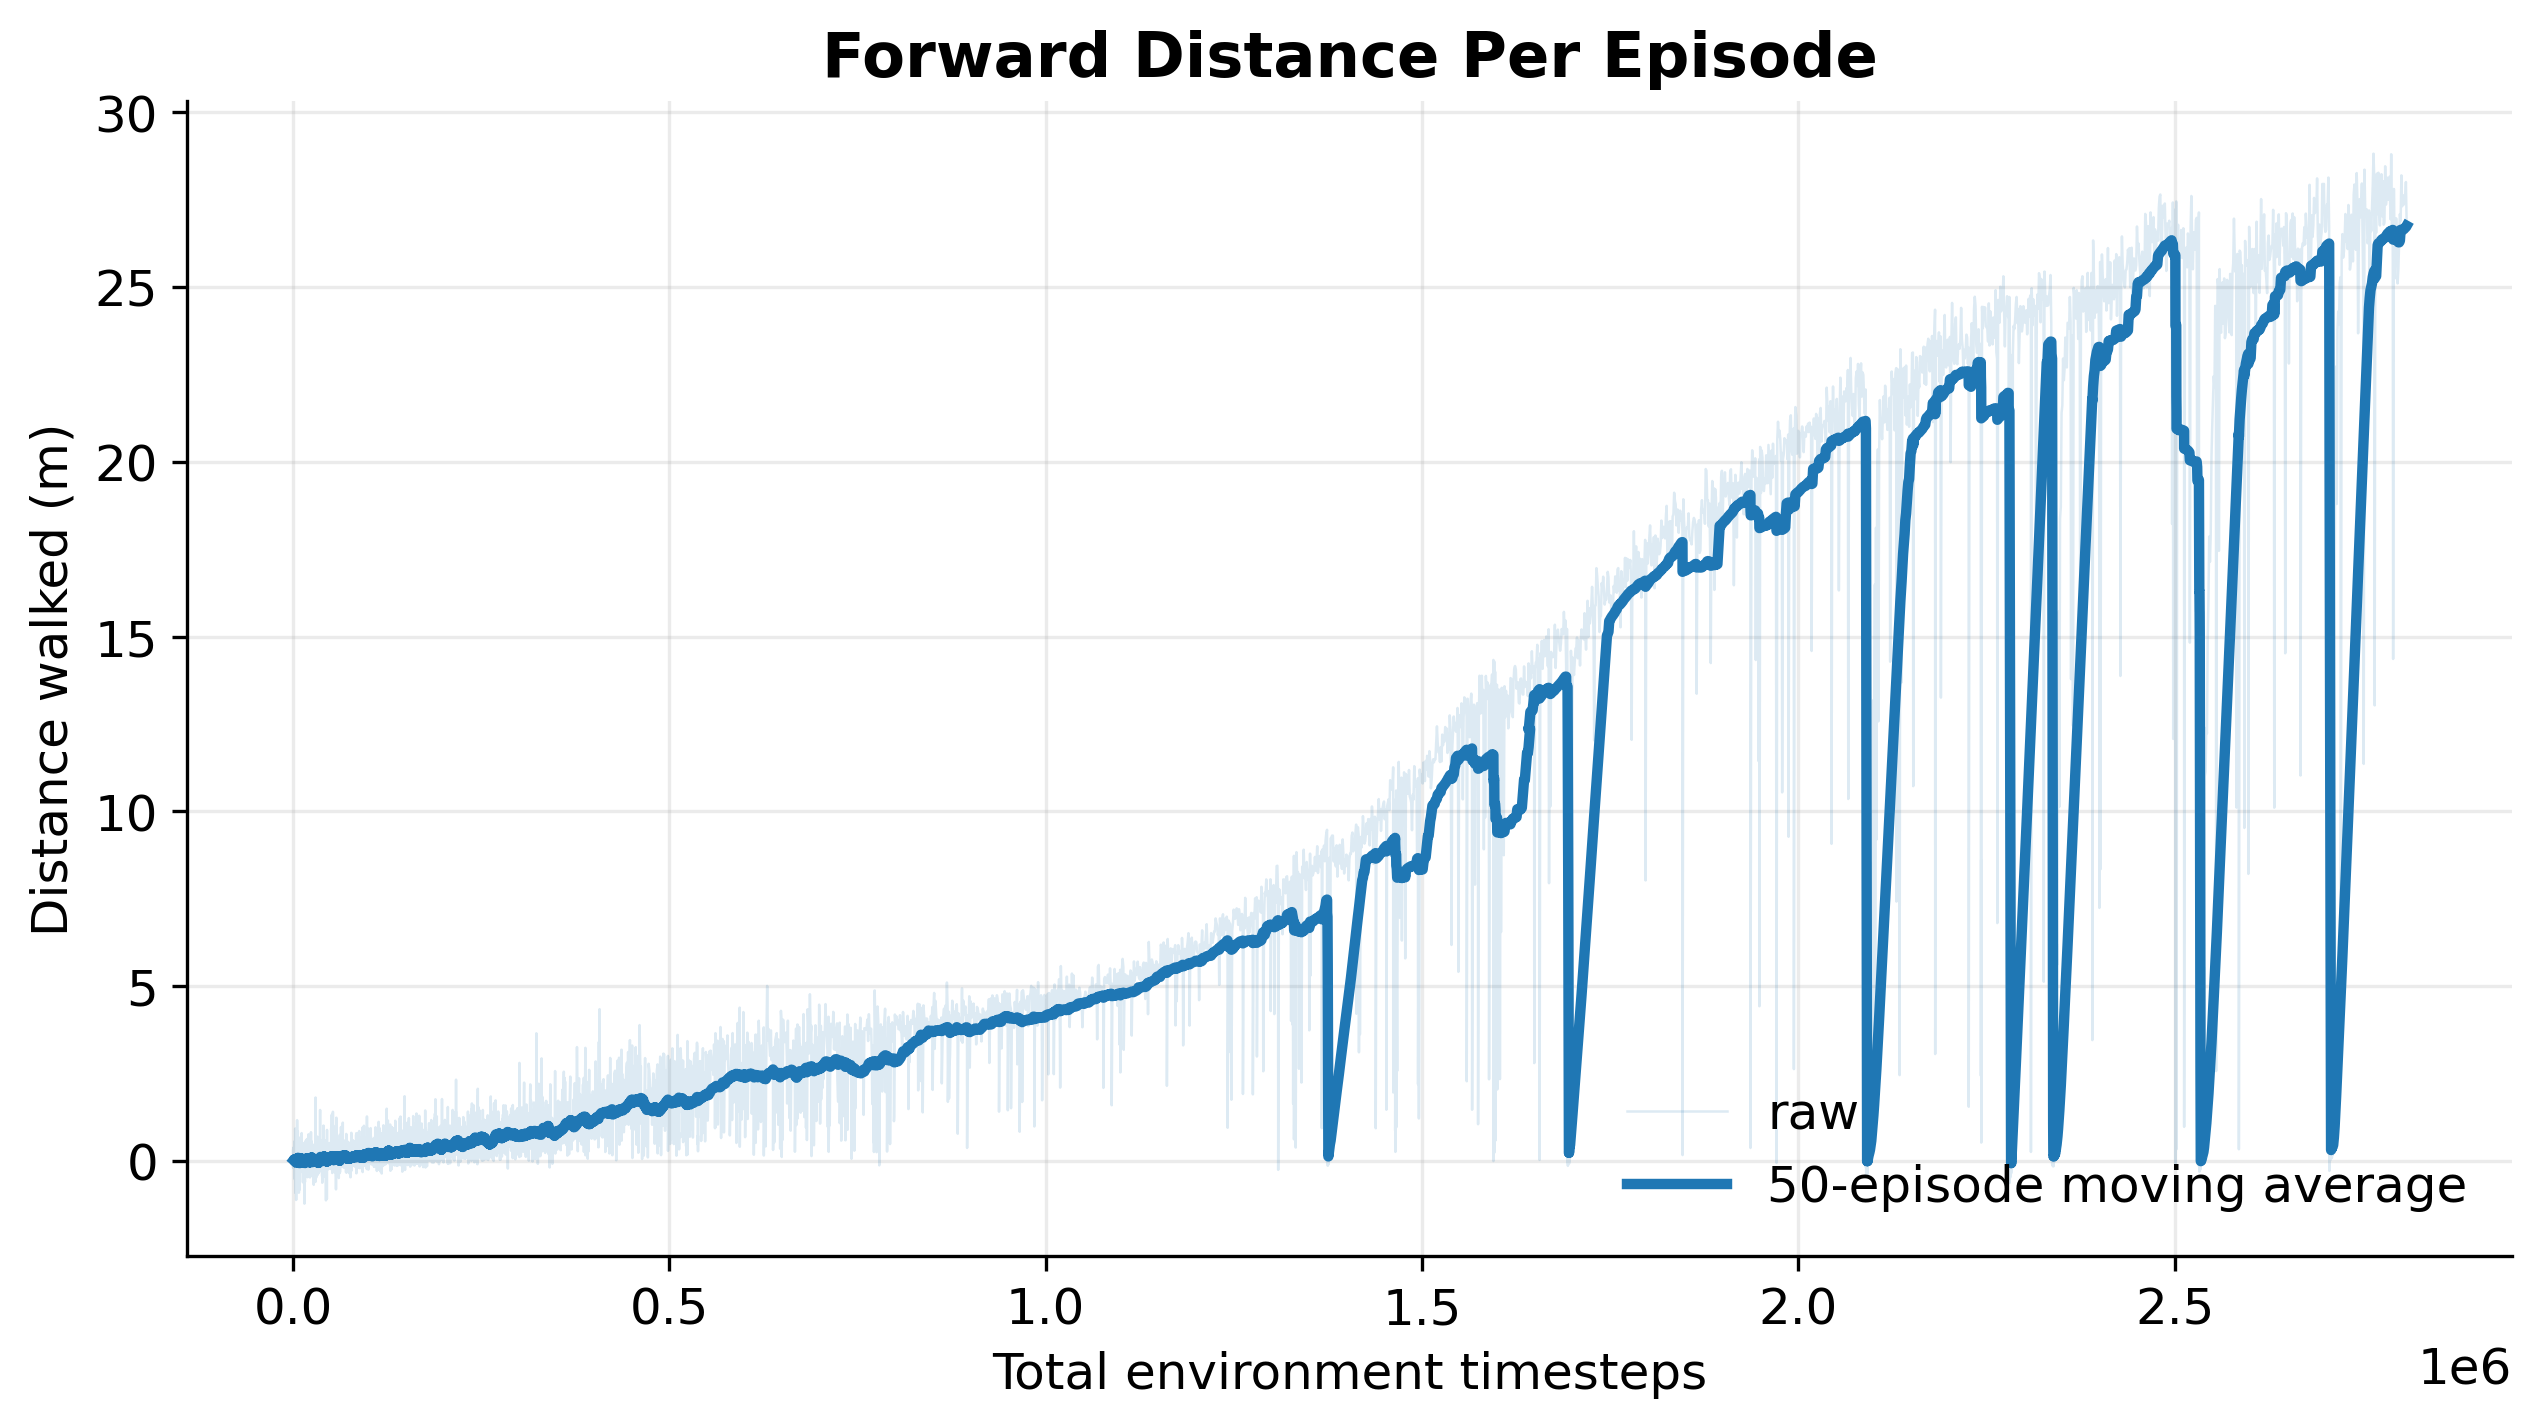
\includegraphics[width=\linewidth]{05_x_distance.png}
  \caption{Forward distance walked per episode. Once the gait emerges the robot
  routinely covers more than 25\,m in a single episode.}
  \label{fig:distance}
\end{figure}

\subsection{Where the reward comes from}
Figure~\ref{fig:reward-mag} plots the mean per-step magnitude of each reward
term over training, and Figure~\ref{fig:pie} gives the same data as a pie
chart over the last 200 episodes. Two things stand out. First, the
forward-velocity term grows monotonically as the policy learns to walk, while
the survival bonus is by definition constant once the episode runs to the
truncation step---together they account for $\sim$82\% of the reward at the
end of training. Second, the energy penalty is a substantial 12\% of the
final reward. We tried smaller energy weights and the policy converged to a
behavior that ``shimmered'' the legs at high frequency: it scored well on
forward velocity but used roughly twice the torque per meter. The current
weight balances those terms reasonably well.

\begin{figure}[t]
  \centering
  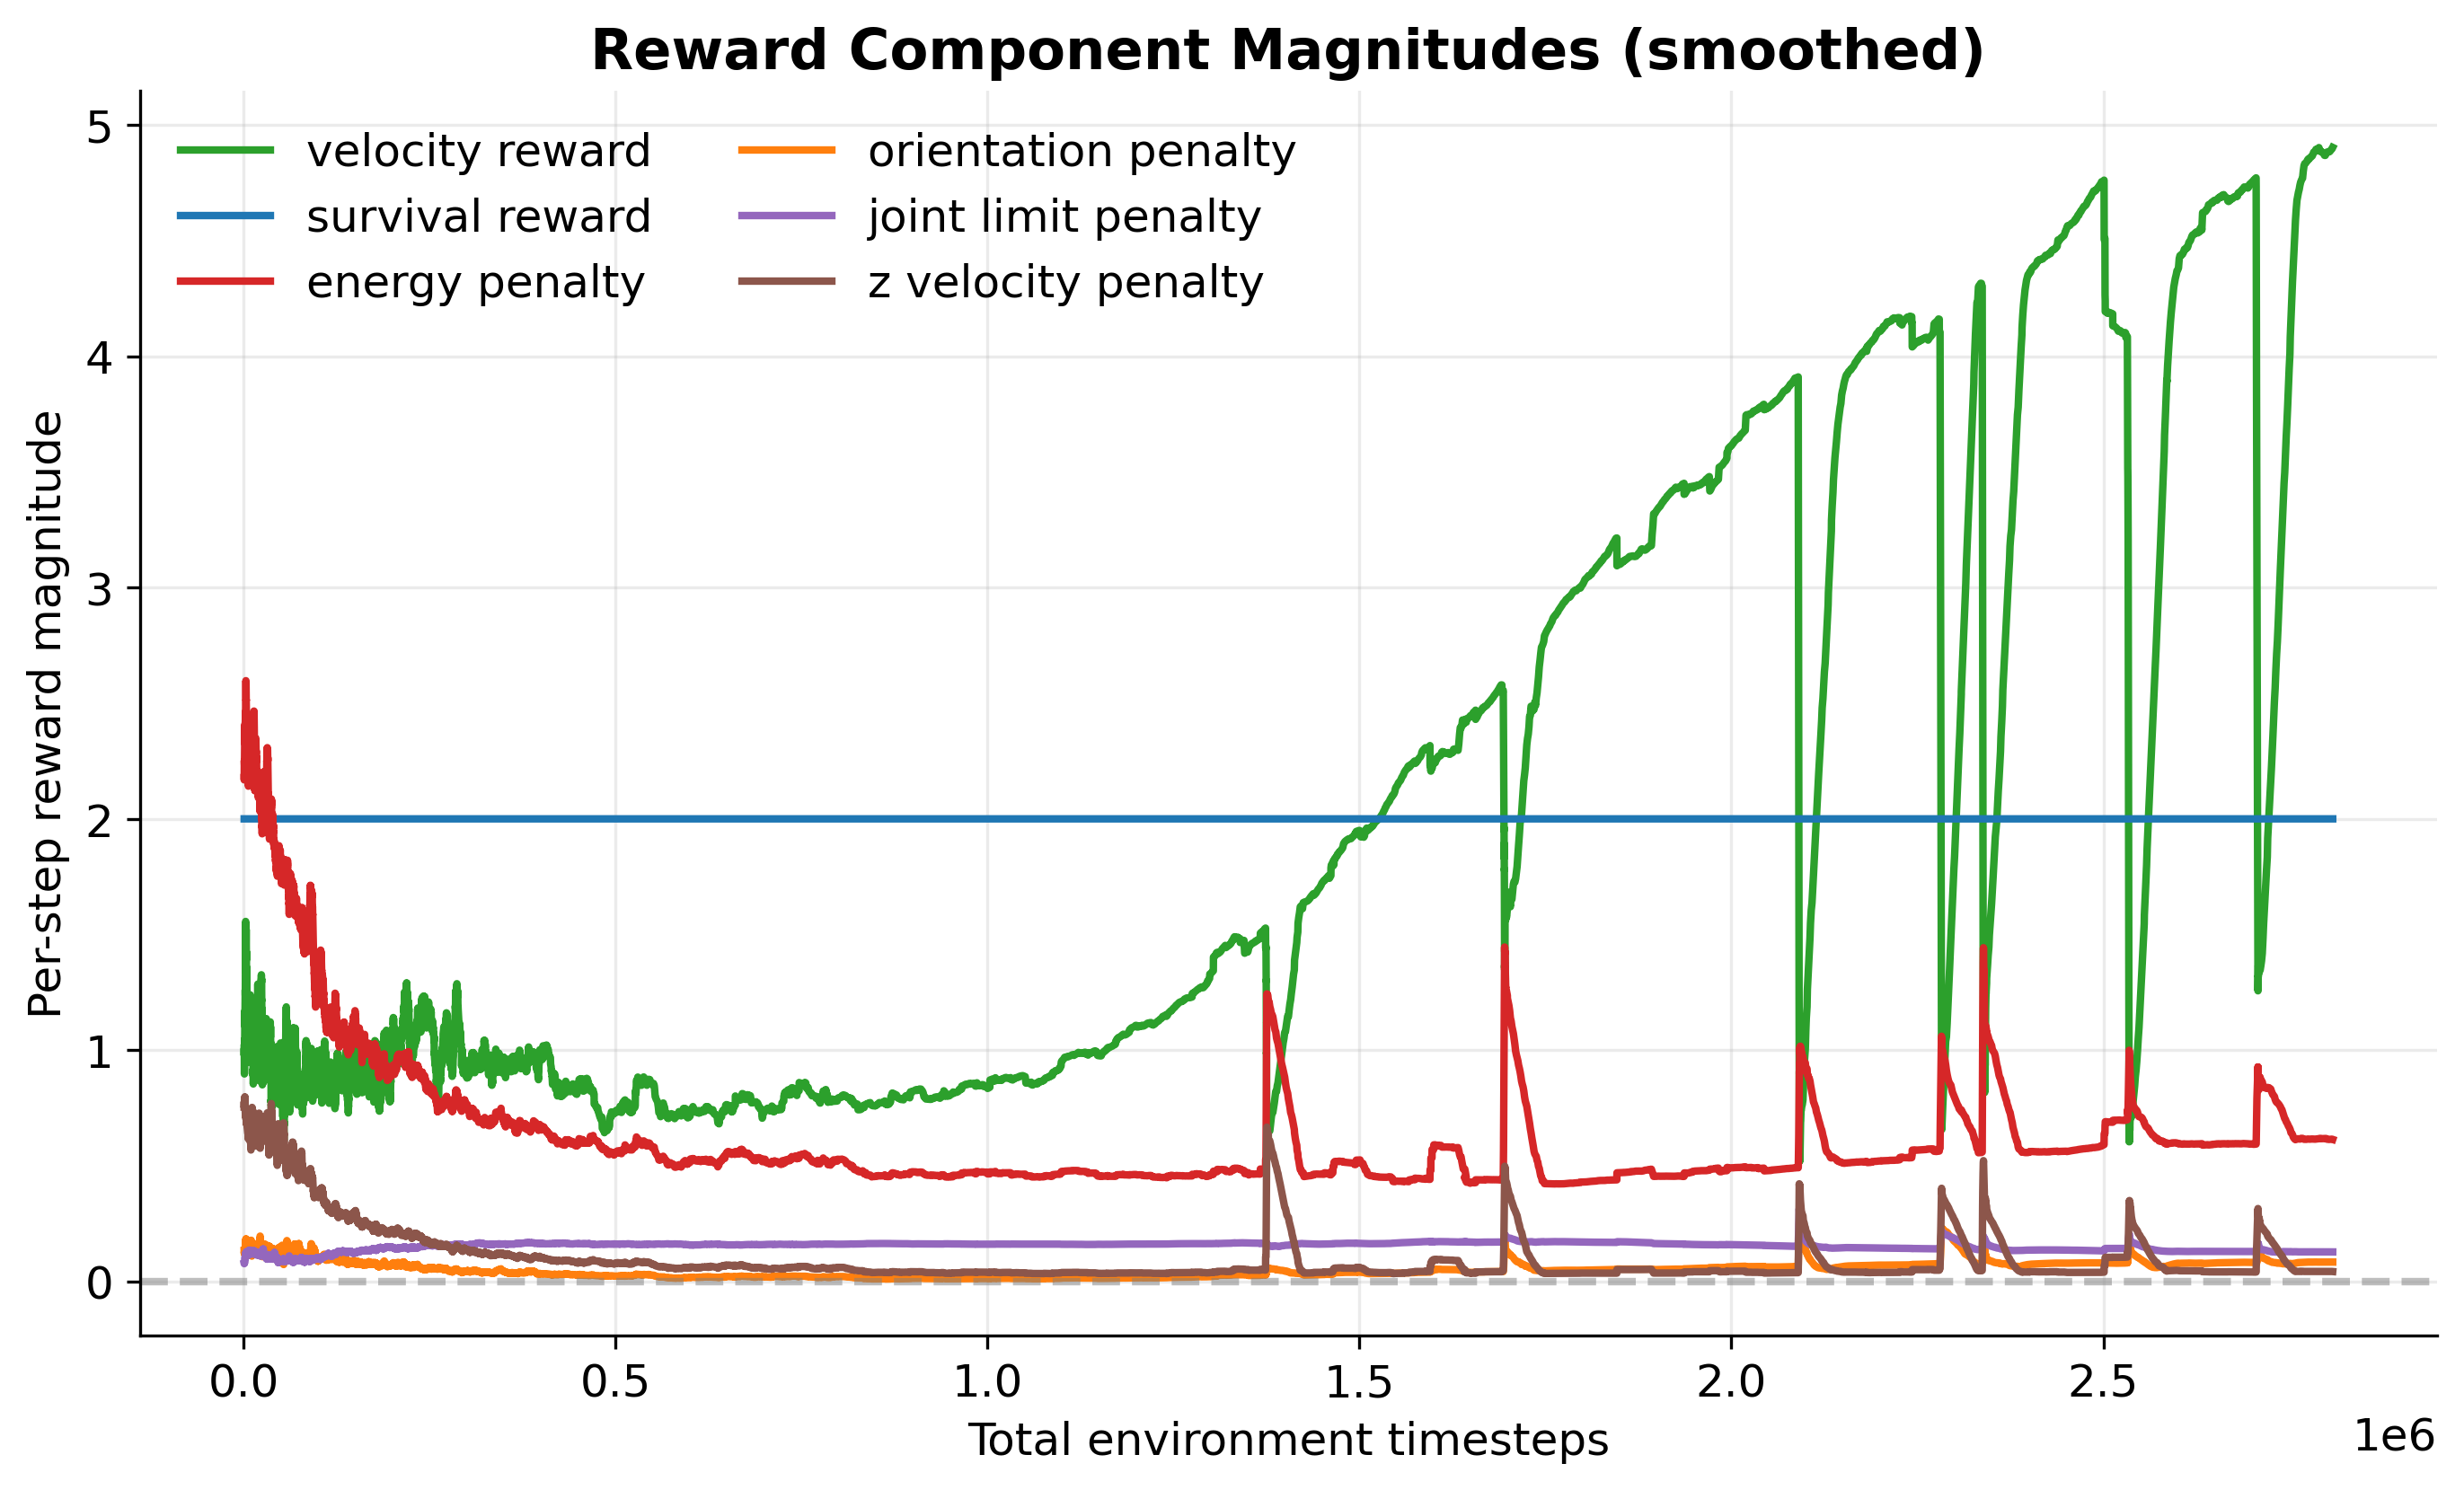
\includegraphics[width=\linewidth]{06_reward_components.png}
  \caption{Mean per-step magnitude of each reward term over training. Forward
  velocity (green) takes over once standing is solved.}
  \label{fig:reward-mag}
\end{figure}

\begin{figure}[t]
  \centering
  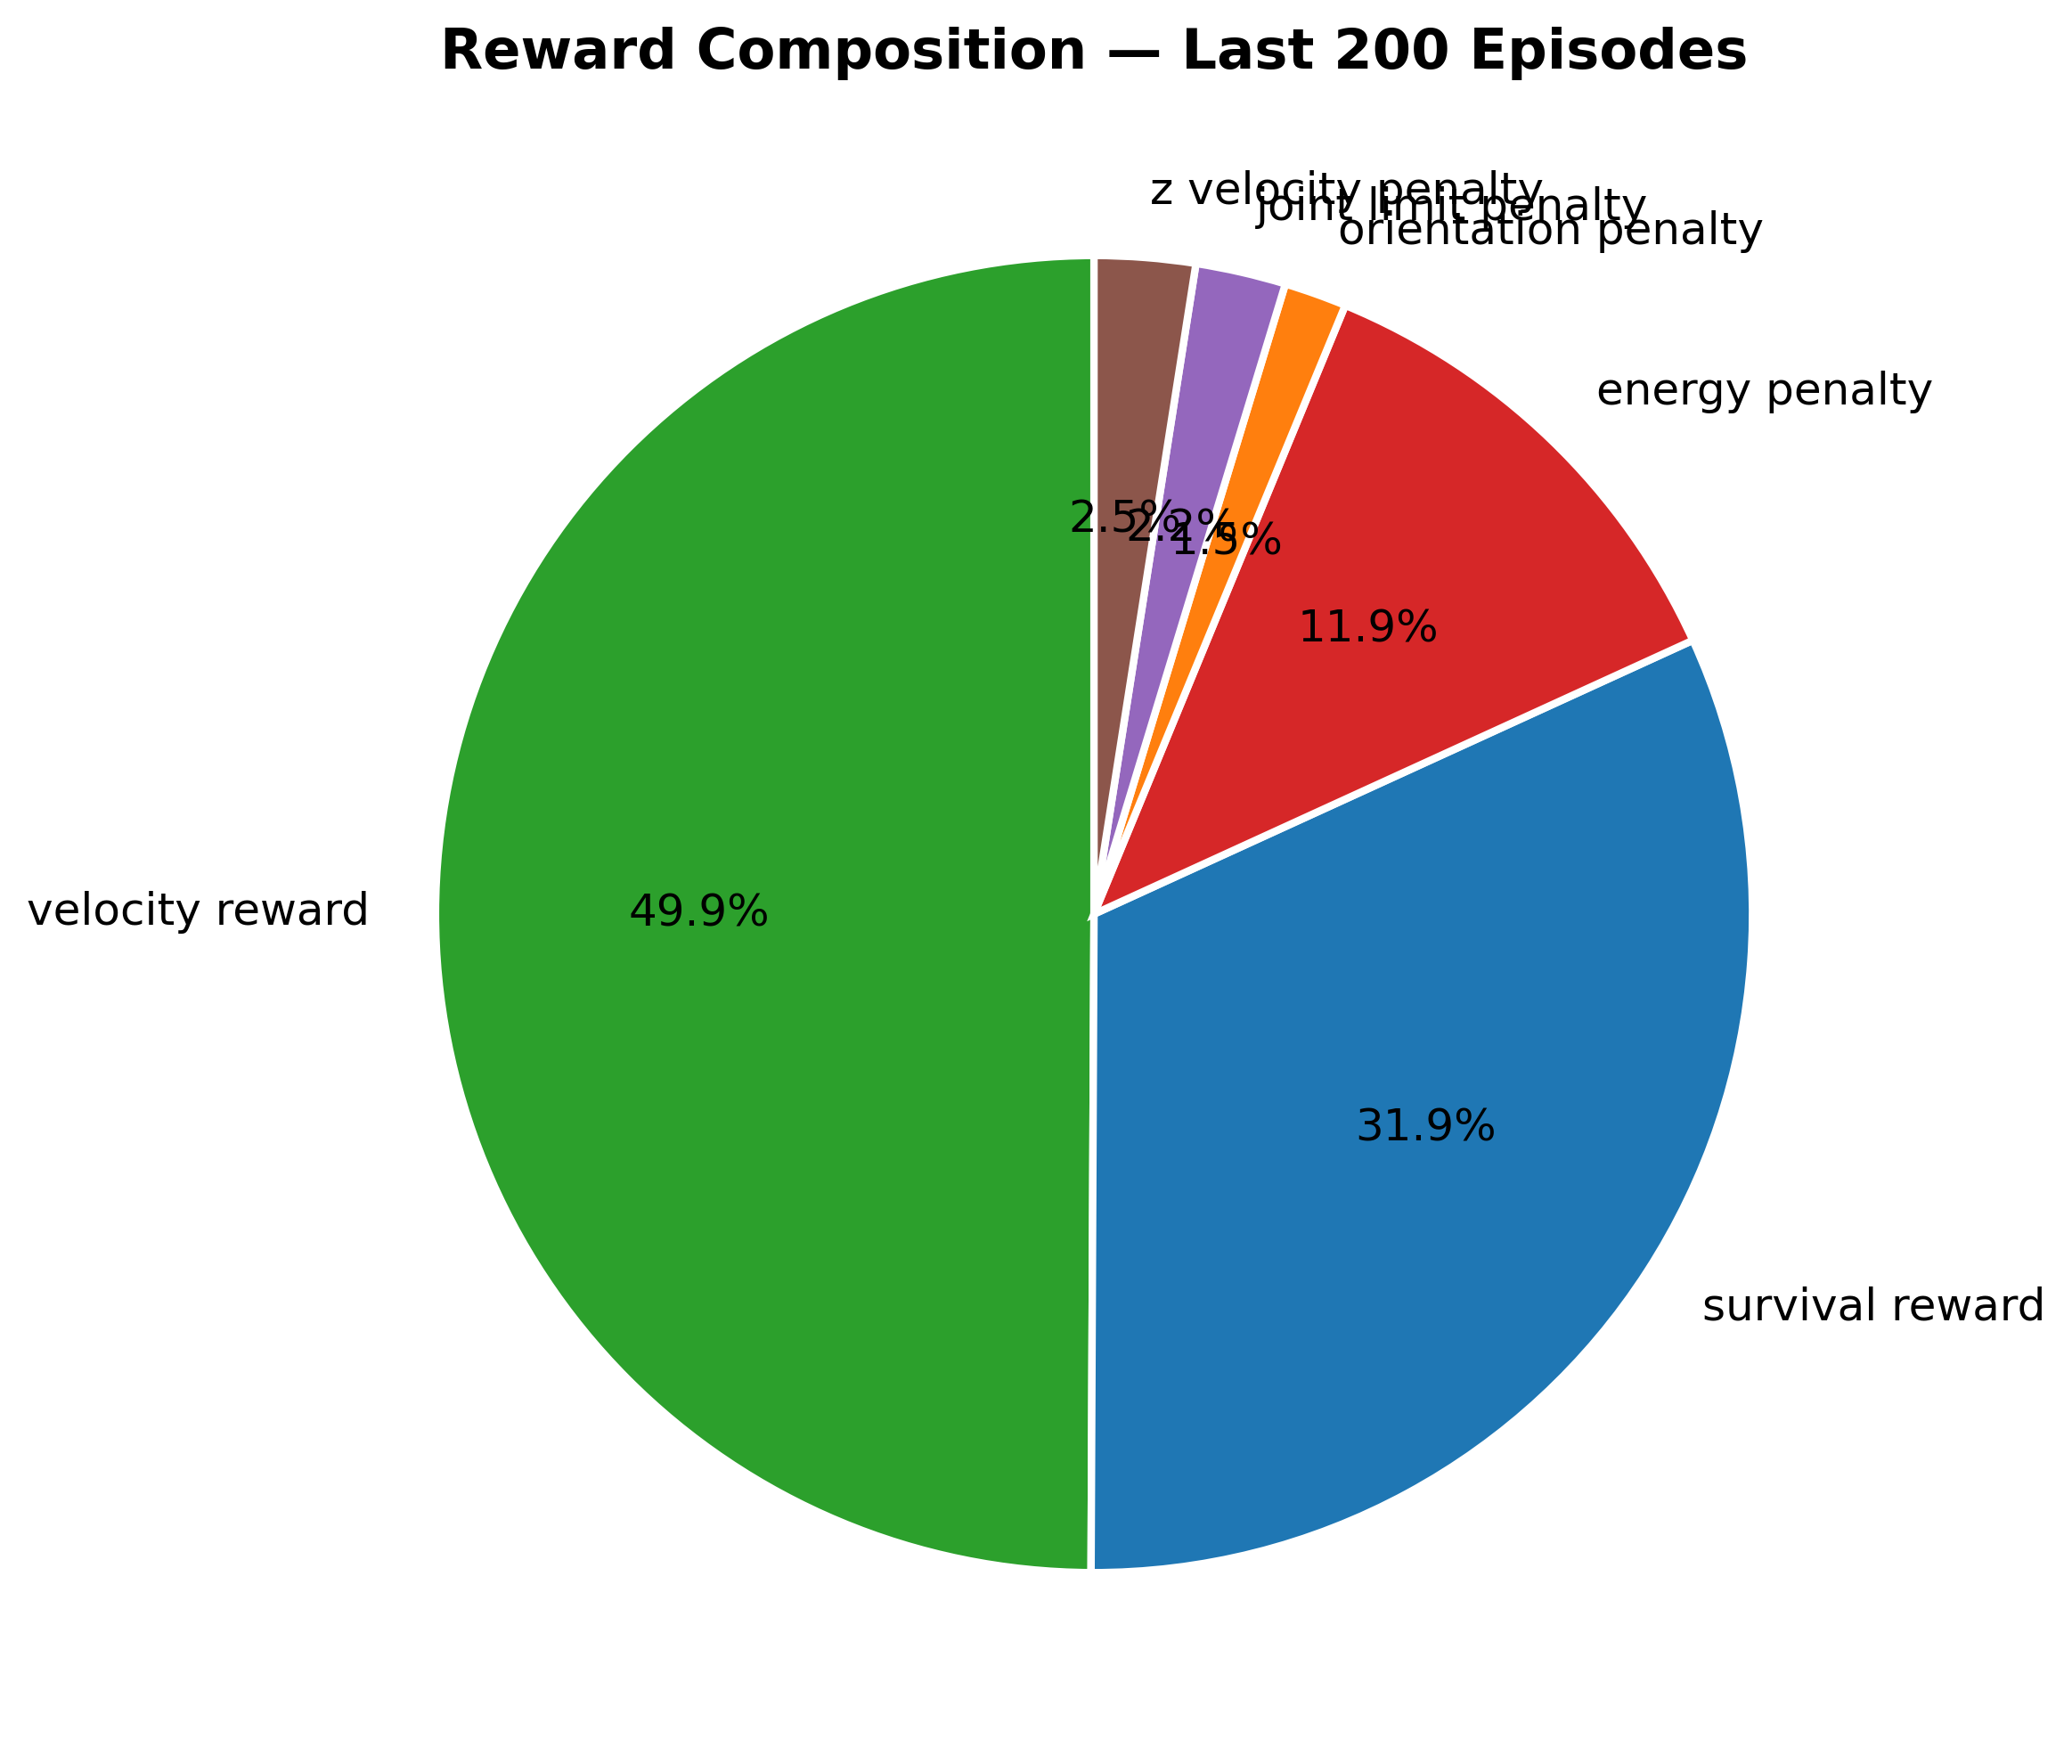
\includegraphics[width=0.85\linewidth]{07_component_pie.png}
  \caption{Reward composition over the last 200 episodes. Velocity and survival
  dominate; the energy penalty is the next largest term.}
  \label{fig:pie}
\end{figure}

Figure~\ref{fig:rewdist} shows the distribution of episode returns over the
first 25\% versus the last 25\% of episodes. Early returns cluster near zero
(robot falls immediately, no velocity); late returns are bimodal with a heavy
peak around 5{,}000--6{,}500 and a small tail near zero corresponding to the
forgetting events.

\begin{figure}[t]
  \centering
  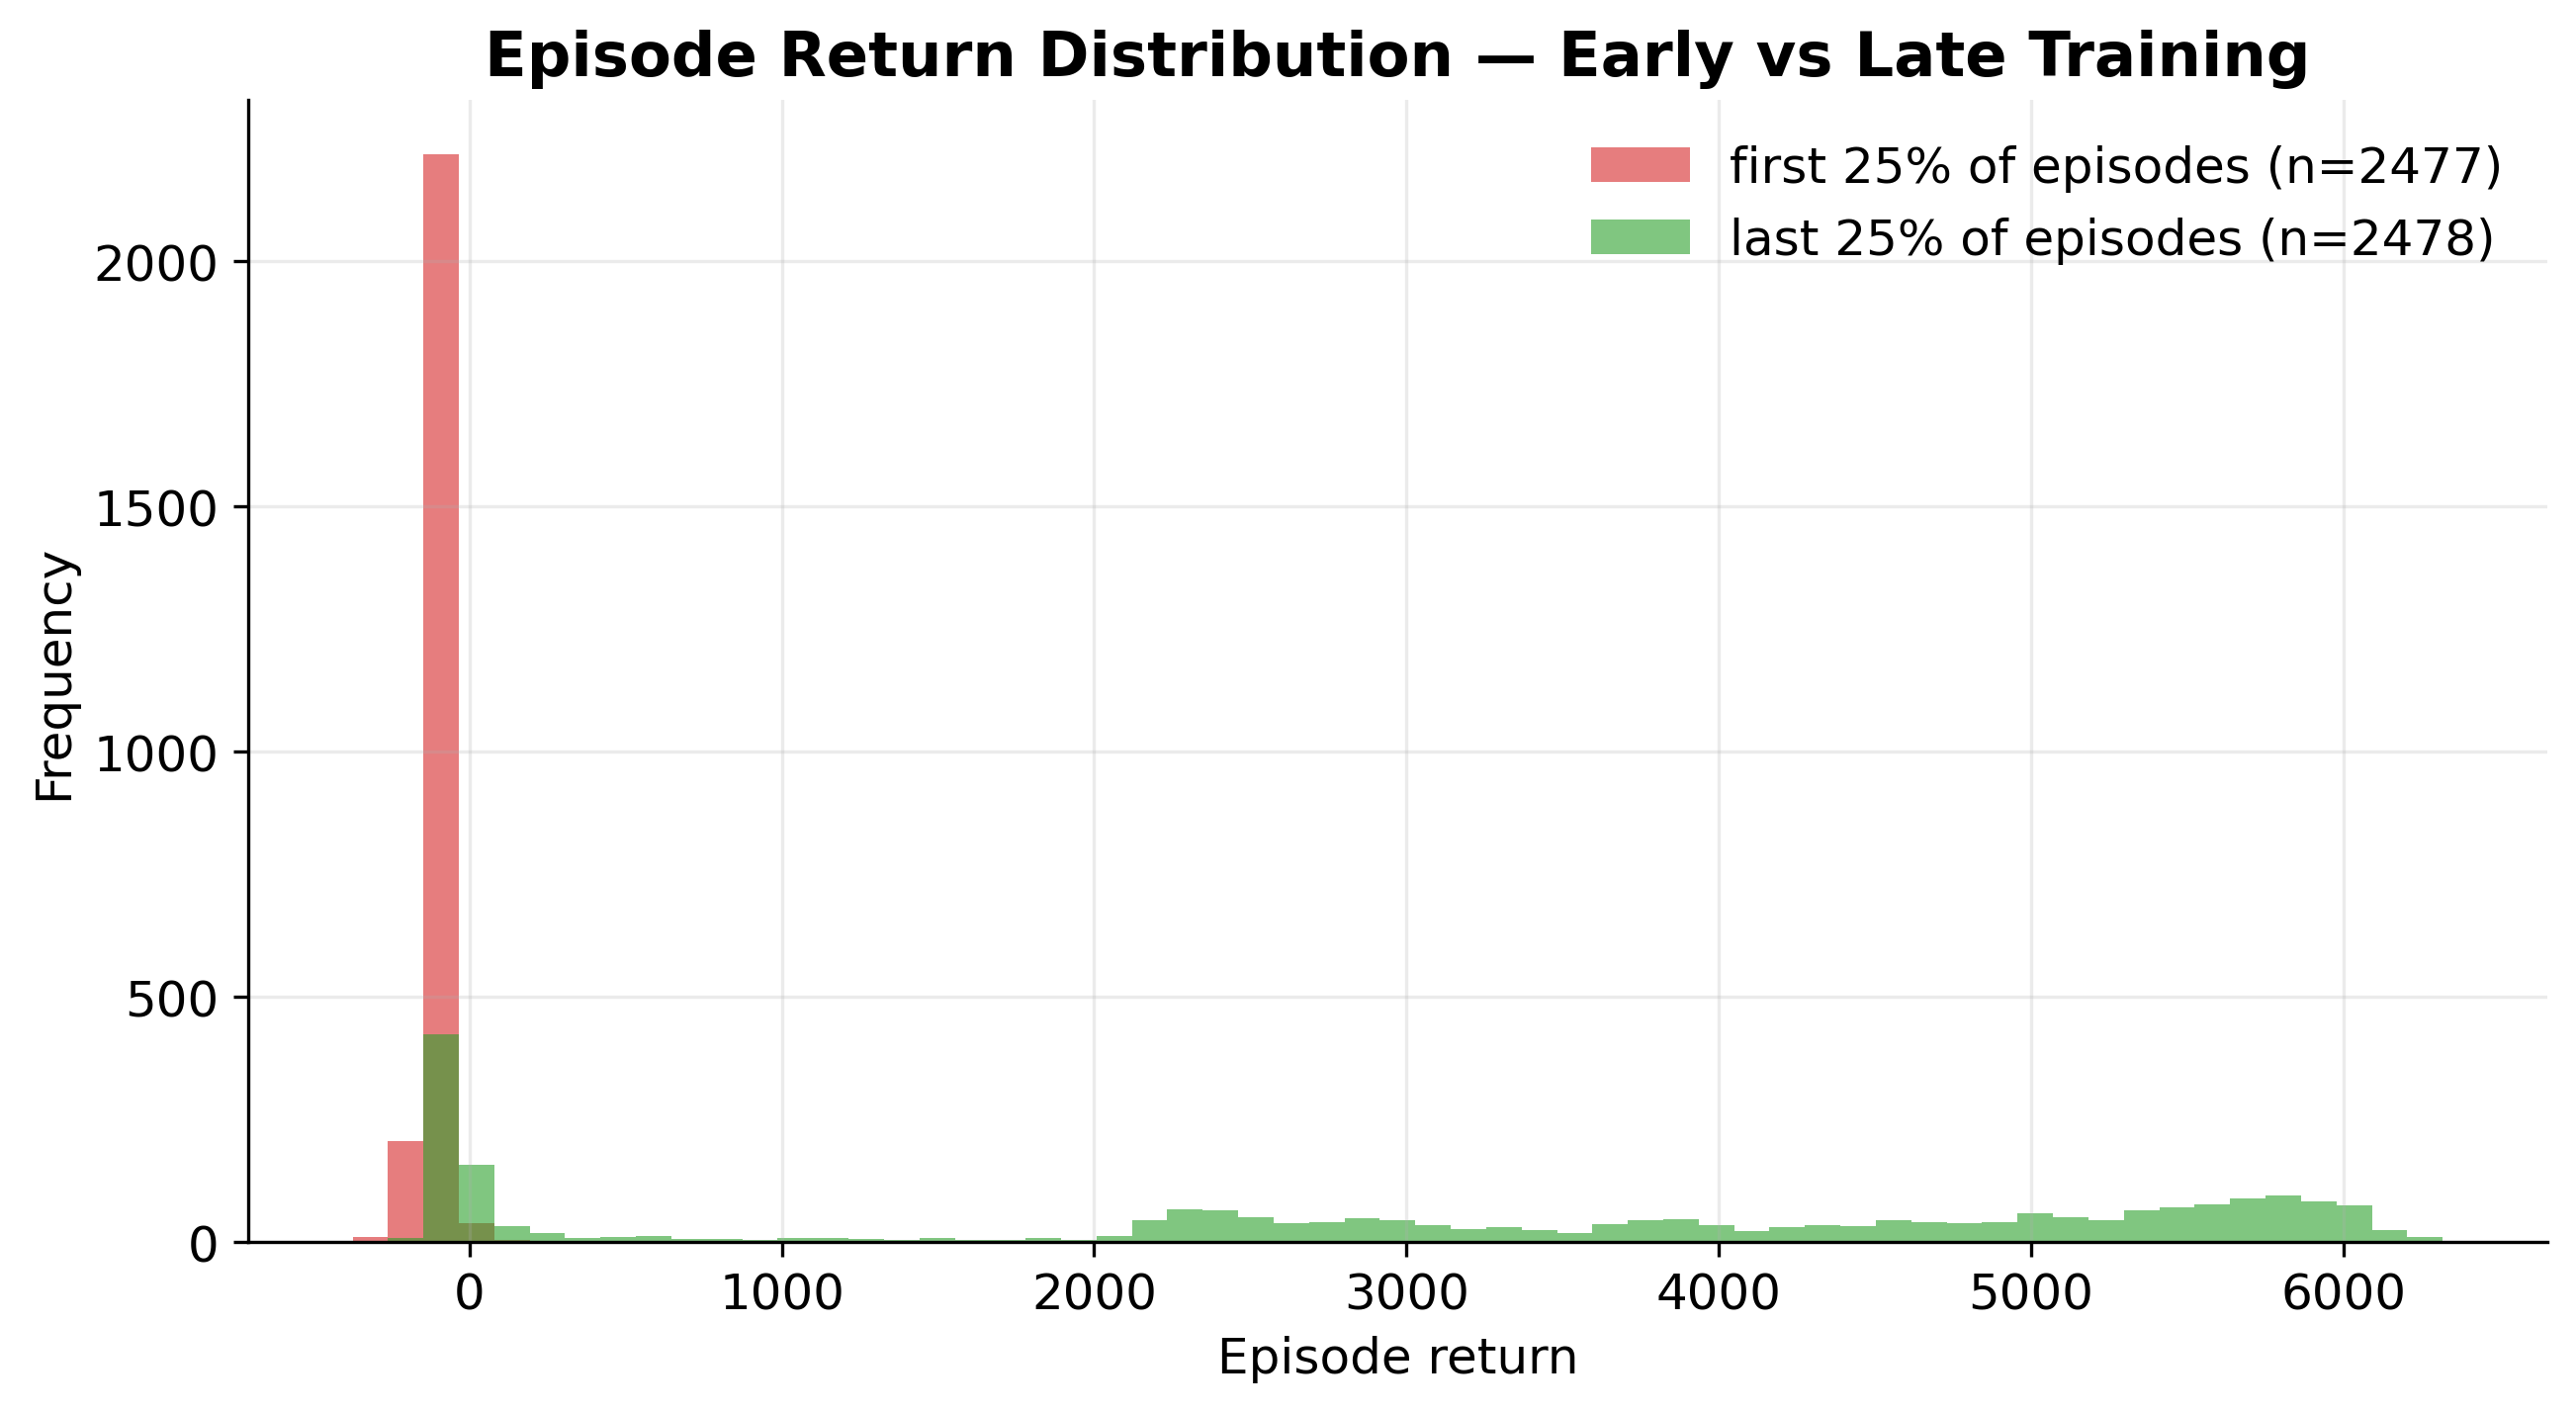
\includegraphics[width=\linewidth]{10_reward_distribution.png}
  \caption{Histogram of per-episode returns, comparing the first 25\% (red)
  and last 25\% (green) of training episodes.}
  \label{fig:rewdist}
\end{figure}

\subsection{Auto-tuned entropy}
SAC adapts an entropy coefficient $\alpha$ to keep the policy near a target
entropy of $-5$. Figure~\ref{fig:alpha} shows $\alpha$ on a log scale. After a
brief spike during the first $\sim$50\,k transitions while the buffer fills,
$\alpha$ drops two orders of magnitude and then very slowly anneals further as
the policy commits to a gait. The small spikes near the end of training match
the catastrophic-forgetting dips: when the policy collapses, returns drop, the
target-entropy controller pushes $\alpha$ up to encourage re-exploration, and
the policy re-learns standing from the replay buffer.

\begin{figure}[t]
  \centering
  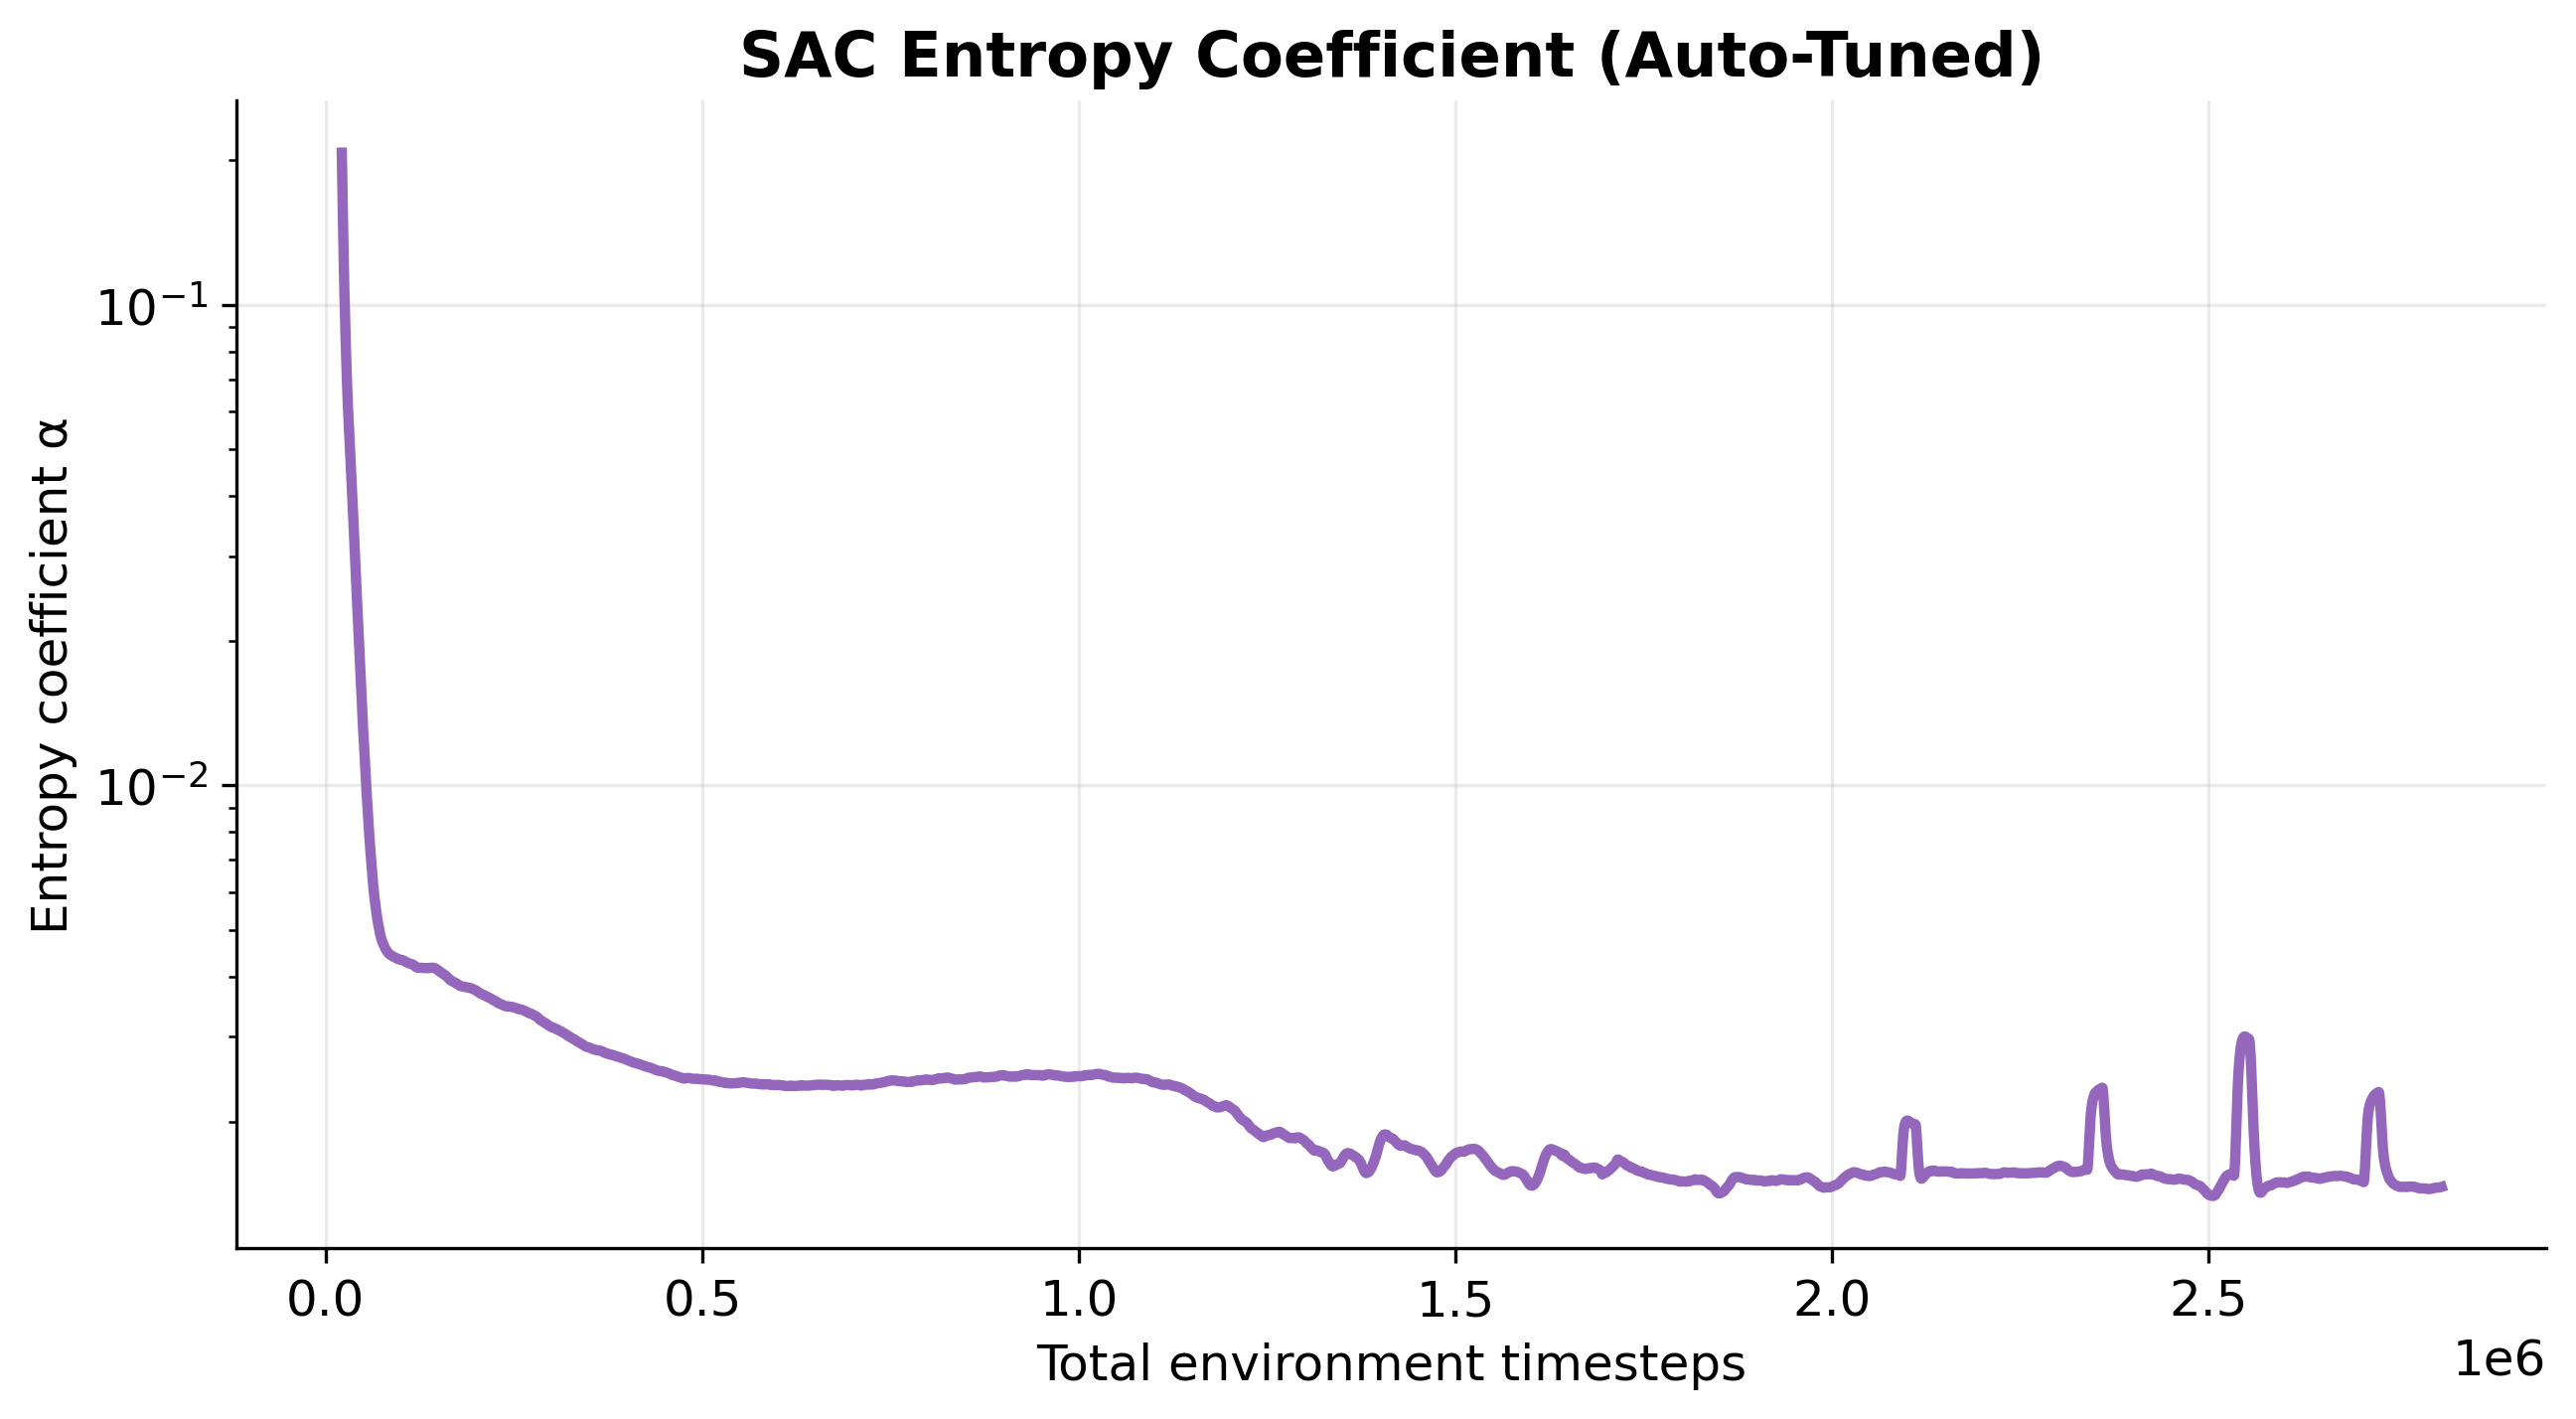
\includegraphics[width=\linewidth]{09_entropy_coef.png}
  \caption{SAC's auto-tuned entropy coefficient $\alpha$ (log scale). The
  small bumps after 2\,M steps are the controller responding to brief policy
  collapses.}
  \label{fig:alpha}
\end{figure}

\subsection{PPO results}
\textit{Note: PPO TensorBoard logs are not in the same directory tree as the
SAC metrics, so the figures referenced here are the screenshots taken from our
in-class presentation; the underlying numbers are summarized in
Table~\ref{tab:compare}.}

PPO never reached SAC's level on this task. Across five reward variants and a
1.4\,M-step run we capped the best evaluation return around 3{,}000, and most
runs plateaued well below that. Two failure modes were common:

\begin{itemize}
\item \textbf{Reward hacking the survival term.} With a high survival bonus
  the policy quickly converged to a stationary T-pose: it satisfied every
  termination check, collected the alive bonus for 1{,}000 steps, and never
  attempted to walk. Lowering the survival weight or scaling up the velocity
  term recovered movement, but in the next iteration the policy would tip
  forward and ``fall walk'' for a few steps before terminating.
\item \textbf{No lateral-motion penalty.} Early PPO runs rewarded torso
  $\dot{x}$ without penalizing $\dot{y}$; the policy responded by walking
  diagonally, exploiting the fact that any positive $x$-component still
  scored. We patched the reward but PPO did not have time to retrain to the
  same level as SAC.
\end{itemize}

\begin{table}[t]
\caption{Final PPO vs.\ SAC comparison.}
\label{tab:compare}
\begin{tabular}{lll}
\toprule
                 & PPO            & SAC \\
\midrule
On / off policy  & on             & off \\
Replay buffer    & --             & 1\,M \\
Steps trained    & $\sim$1.4\,M   & $\sim$2.8\,M \\
Best eval return & $\sim$3{,}000  & $\sim$7{,}100 \\
Best fwd speed   & $\sim$0.4\,m/s & $\sim$1.6\,m/s \\
Throughput       & $\sim$300 sps  & $\sim$50 sps \\
\bottomrule
\end{tabular}
\end{table}

\subsection{Failure modes and limitations}
A few qualitative observations are worth recording, since they would shape any
follow-up work:

\textbf{Catastrophic forgetting.} Long SAC runs are not monotonic. After the
robot has been walking reliably for hundreds of thousands of steps, it can
abruptly lose its balance for a few episodes and collapse the return curve to
nearly zero before recovering. The dips are visible in
Figs.~\ref{fig:learning-curve}, \ref{fig:survival}, and \ref{fig:distance}. We
suspect the cause is the replay buffer slowly ageing out the
``early-fall'' transitions: once the buffer contains almost only successful
walking trajectories, a small policy update can move into a region the critic
has not seen in a long time, and the policy chases a stale gradient briefly
before the entropy controller pushes exploration back up. Periodically mixing
in older transitions or using a smaller learning rate late in training would
likely fix this.

\textbf{Unconventional gaits.} The robot did not converge to a clean
human-style heel-toe gait. The final policy uses what looks more like a duck
walk: knees stay bent, ankles push off in a short hop, and the torso leans
slightly forward. This is a legitimate local optimum of the reward---it scores
well on velocity, survival, and energy. Without a periodic phase reward or a
motion-capture imitation term~\cite{peng2018deepmimic}, there is no signal
encouraging a particular limb-coordination pattern.

\textbf{Locked arms.} Holding the arms at zero simplifies training but also
removes a useful degree of freedom for balance. Re-running with the full
21-joint action space is straightforward but would significantly change
the credit-assignment problem.

\textbf{Sim-to-real gap.} We never deploy on the physical T1, so all numbers
are simulation-only. Domain randomization (motor friction, link mass, latency)
would be a natural next step before any hardware test.

\subsection{Ethical considerations}
The system here is a small humanoid in a single, flat simulation environment;
the ethical scope is correspondingly narrow. Two issues are nonetheless
worth flagging. First, learned locomotion controllers can encode unsafe
behaviors that are hard to detect from training metrics alone (for instance, a
policy that scores well on forward velocity but slams its feet into the ground
hard enough to damage real hardware). Standard deployment hygiene---
torque/velocity limits, hardware estops, and behavior-clone fallbacks---is
sufficient to mitigate this in a research setting. Second, robots that walk
reliably are dual-use; we are studying an academic platform but the same
techniques are common in surveillance and military contexts. We do not view
our specific contribution as moving that frontier, but flag it for
completeness.

% ====================================================================
\section{Conclusion and Future Work}\label{sec:conclusion}
% ====================================================================
We trained a 13-DoF bipedal humanoid to walk in PyBullet using two standard
deep-RL algorithms and a hand-shaped reward. SAC produced a stable forward
gait at $\sim$1.6\,m/s after $\sim$2.8\,M environment steps; PPO under the
same wall-clock budget plateaued at less than half of SAC's return. The
biggest practical lesson from the project is how much of the work is in the
reward function rather than the algorithm: small changes to the survival
bonus or the energy weight produced very different gaits, and most of the
time we spent debugging was actually time spent diagnosing reward hacks.

If we had another month we would: (1) add domain randomization and a
sim-to-real test on the physical T1 platform; (2) re-introduce the arm joints
into the action space, since arm motion is critical for human walking and may
help SAC stabilize at higher speeds; (3) replace the dense forward-velocity
reward with a target-velocity tracking reward so the policy can be commanded
at run time; (4) add a periodic gait reward or short imitation reference to
encourage symmetric stepping; and (5) parallelize rollouts (e.g.\ Isaac
Gym~\cite{rudin2022learn}) so a full PPO sweep takes hours rather than days.

% ====================================================================
\section{Contribution Statement and Peer Evaluation}\label{sec:contributions}
% ====================================================================
All three authors contributed substantively to the project. A short summary
of individual contributions is below; the team agrees that contributions were
roughly equivalent in effort, with the breakdown reflecting areas of focus
rather than relative workload.

\begin{description}
\item[Drew Burcher] Set up the PyBullet/Gymnasium environment and the
  Stable-Baselines3 training harness, including the auto-commit/metadata
  pipeline, the live training dashboard, and the evaluation/GIF recorder.
  Ran and tuned the SAC experiments and produced all SAC plots used in
  Section~\ref{sec:results}.
\item[Dan Torri] Led the PPO experiments: implemented the multiple
  reward-weight variants, ran the long PPO sweep, and produced the PPO
  TensorBoard plots and qualitative analysis. Drafted the related-work
  section and the PPO/SAC comparison.
\item[Nathan Wyatt] Designed and iterated on the reward function (especially
  the energy, joint-limit, and z-velocity terms), implemented the reward
  ablation script, and contributed the methodology and ethical-considerations
  text. Coordinated meetings and slide preparation for the in-class
  presentation.
\end{description}

\paragraph{Peer evaluation.}
Each member rates the other two as fully meeting expectations on attendance,
follow-through, and code/writing quality. There were no disputes during the
project. We make no asymmetric peer-evaluation claims.

\bibliographystyle{ACM-Reference-Format}
\bibliography{refs}

\appendix

\section{Hyperparameters}
Table~\ref{tab:hparams} lists the algorithm hyperparameters used for the runs
reported in Section~\ref{sec:results}. All values match the
\texttt{config.py} file in the project repository.

\begin{table}[!htbp]
\caption{SAC and PPO hyperparameters used in the reported runs.}
\label{tab:hparams}
\begin{tabular}{lll}
\toprule
                 & SAC                   & PPO \\
\midrule
Optimizer        & Adam                  & Adam \\
Learning rate    & $3\times10^{-4}$      & $3\times10^{-4}$ \\
Discount $\gamma$ & 0.99                 & 0.99 \\
Network          & MLP $[256,256]$       & MLP $[256,256]$ \\
Batch size       & 256                   & 64 \\
Replay buffer    & $10^6$                & --- \\
Soft update $\tau$ & 0.005               & --- \\
Target entropy   & $-5$ (auto $\alpha$)  & --- \\
Rollout length   & ---                   & 2{,}048 \\
Epochs / update  & ---                   & 10 \\
GAE $\lambda$    & ---                   & 0.95 \\
Clip range       & ---                   & 0.2 \\
Entropy coef     & ---                   & 0.01 \\
Value coef       & ---                   & 0.5 \\
\bottomrule
\end{tabular}
\end{table}

\section{Reward weights}
Table~\ref{tab:rewards} lists the per-term reward weights used for the SAC run
reported in Section~\ref{sec:results}. The reward formula is given in
Section~\ref{sec:method}.

\begin{table}[!htbp]
\caption{Reward weights for the reported SAC run.}
\label{tab:rewards}
\begin{tabular}{ll}
\toprule
Term                  & Weight \\
\midrule
Forward velocity      & $+3.0$ \\
Survival (alive)      & $+2.0$ \\
Energy (mean power)   & $-0.00495$ \\
Fall (terminal)       & $-100.0$ \\
Orientation (roll/pitch sq.) & $-0.5$ \\
Joint-limit (excess sq.)     & $-0.2$ \\
Z-velocity (downward) & $-0.5$ \\
\bottomrule
\end{tabular}
\end{table}

\end{document}
